\chapter{Materiales y métodos}
\section{Marco teórico}
\subsection{Sistema de reconocimiento de voz}

\subsubsection{Historia del reconocedor de voz}
Todo empezó con Alexander Graham Bell en los años 1870’s, el quería construir un dispositivo que hiciera el habla visible a las personas con problemas auditivos, el cual tuvo como resultado el teléfono. Luego años más tarde en 1910’s, AT\&T Bell Laboratories, construye la primera máquina capaz de reconocer voz basada en plantillas de los 10 dígitos en inglés. Requería un extenso reajuste a la voz de una persona, pero una vez logrado tenía un 99\% de certeza. Por lo tanto, surge la esperanza de que el reconocimiento de voz es simple y directo, \citep{eyra}.
\vskip 0.5cm
En 1940’s y 1950’s, la mayoría de los investigadores reconocen que era un proceso mucho más intrincado y sutil de lo que habían anticipado. Por lo tanto, empiezan a reducir los alcances y se enfocan a sistemas más específicos: dependientes del locutor, flujo discreto del habla (con espacios o pausas entre palabras) y de vocabulario pequeño (menor o igual a 50 palabras), \citep{eyra}.
\vskip 0.5cm
Estos sistemas empiezan a incorporar técnicas de normalización del tiempo (minimizar diferencia en velocidad del habla). Además, ya no buscaban una exactitud perfecta en el reconocimiento. Después IBM y CMV trabajan en reconocimiento de voz continuo, pero no se ven resultados hasta los 1970’s, \citep{eyra}.
\vskip 0.5cm
En 1970’s, un ambicioso proyecto para construir un sistema informático que entienda y procese el habla fue iniciado por DARPA, la meta era integrar conocimiento acerca del habla, lingüística e inteligencia artificial para desarrollar un \textit{Sistema Informático del Lenguaje Hablado}. Se desarrolló un sistema informático llamado \textit{Harpy} que integraba todas las fuentes de conocimiento en redes de estado finito, que eran entrenadas estadísticamente. En estos años crecen notoriamente métodos que hacen uso de la probabilidad y se entiende por \textit{Reconocimiento Automático del Habla} como buscar la palabra más probable en una señal de audio, dada alguna información de su distribución de probabilidad, \citep{orlando}.
\vskip 0.5cm
En 1980’s, modernos reconocedores son lanzados al mercado, los algoritmos desarrollados en este tiempo son usados todavía en estos días como: Modelos n-grams, Mixturas Gaussianas, Modelos Ocultos de Markov, Decodificador Viterbi, etc. En 1984 es construido el primer sistema de dictado en tiempo real, por IBM, \citep{orlando}.
\vskip 0.5cm
En 1990’s, con el aumento del poder de cómputo y capacidad de memoria de las computadoras existen avances en algoritmos de adaptación y entrenamiento discriminativo, a la vez se desarrollan sistemas informáticos que reconocían palabras independientemente quien fuera el hablante, algunas de estas aplicaciones fueron implantadas en empresas telefónicas. En 1995, Dragon IBM lanza su producto que reconocía palabras aisladas dependiente del hablante, era un sistema que permitía un dictado de un gran número de palabras. Dos años más tarde lanzaron su sistema para dictado continuo. En 2000’s, teléfonos celulares ya ofrecían servicios de marcado activado por voz, \citep{orlando}.
\vskip 0.5cm
En los años 2010’s, salió a la luz el asistente de voz Siri, realizando funciones de un asistente personal para dispositivos iOS, macOS, tvOS y watchOS. Esta aplicación utiliza procesamiento del lenguaje natural para responder preguntas, hacer recomendaciones y realizar acciones mediante la delegación de solicitudes hacia un conjunto de servicios web. También surgieron asistentes de voz como Cortana de Microsoft y Alexa de Amazon, \citep{timetoast2010}.
\vskip 0.5cm
En la actualidad, se espera que con el poder de cómputo actual de las máquinas y las diversas investigaciones en el tema, se logre aumentar el desempeño. Aplicaciones actuales van desde software para celulares, robótica hasta interfaces de voz para personas discapacitadas; desafortunadamente las comparaciones de error entre humanos y máquinas todavía dan un amplio margen de diferencia, por lo que se espera lograr que éste margen disminuya en los próximos años.

\subsubsection{Fundamentos sobre sonidos y la señal de voz}
Ahora veremos algunos conceptos empleados en el estudio de las señales de voz, así como en el funcionamiento de los sistemas generadores de voz, de tal forma que se puedan establecer las características que sirvan para realizar un correcto reconocimiento de voz. Existen varias maneras para analizar y describir el habla. Los enfoques más comúnmente usados son:
\begin{enumerate}
\item[•]\textbf{Articulación:} Análisis de cómo el humano produce los sonidos del habla.
\item[•]\textbf{Señal Acústica:} Análisis de la señal de voz como una secuencia de sonidos.
\item[•]\textbf{Percepción Auditiva:} Análisis de cómo el humano procesa el habla.
\end{enumerate}

Los tres enfoques proveen ideas y herramientas para obtener mejores y más eficientes resultados en el reconocimiento.

\begin{enumerate}
\item[a)]Articulación
\par
La voz humana se produce por medio del aparato fonatorio, también llamado aparato bucal o articulatorio, el cual está formado por un conjunto de órganos. El aparato fonador consiste en tres grupos de órganos diferenciados, tal como se ve en la Figura \ref{fig:figura2.1}

\begin{enumerate}
\item[•]\textbf{Órganos de respiración o cavidades infraglóticas:} pulmones, bronquios y tráquea.
\item[•]\textbf{Órganos de fonación o cavidades glóticas:} laringe, cuerdas vocales y resonadores nasal, bucal y faríngeo.
\item[•]\textbf{Órganos de articulación o cavidades supraglóticas:} paladar, lengua, dientes, labios y glotis.
\end{enumerate}

\begin{figure}[ht]
\begin{center}
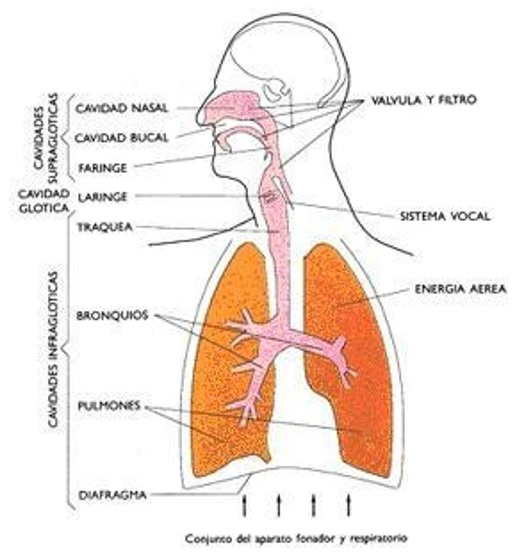
\includegraphics[width=0.4\textwidth]{Imagenes/Cap2/image001}
\end{center}
\begin{center}
\vskip -0.5cm
\caption{\small{Órganos del cuerpo que intervienen en el aparato fonador.}}
\label{fig:figura2.1}
{\small{Fuente: \cite{luis}}}
\end{center}
\end{figure}

El proceso básico de generación de la voz es el mismo ya sea al hablar o al cantar. El cerebro envía señales a través del sistema nervioso a los músculos de la cabeza, cuello y torso de manera que se produzca la inhalación previa a la generación. Al final de la inhalación se efectúan varias acciones, primero se realiza el movimiento de los cartílagos aritenoides en la laringe acercando a las cuerdas vocales entre sí, luego el volumen de los pulmones disminuye para producir una presión de aire positiva en los mismos, después el aire comienza a fluir hacia la laringe generando una excitación y esta adquiere las formas siguientes: fonación, susurro, fricación, compresión y vibración.

\begin{figure}[ht]
\begin{center}
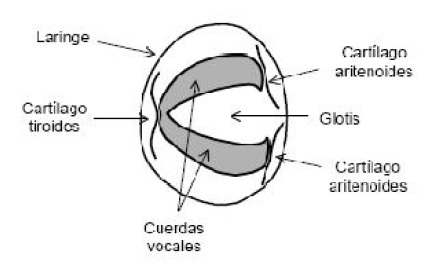
\includegraphics[width=0.4\textwidth]{Imagenes/Cap2/image002}
\end{center}
\begin{center}
\vskip -0.5cm
\caption{\small{Corte esquemático de la laringe en un plano horizontal.}}
\label{fig:figura2.2}
{\small{Fuente: \cite{owens}}}
\end{center}
\end{figure}

Las voces del hombre y la mujer difieren debido a varios aspectos, que incluyen el tamaño de la laringe, el tono, el rango de tono, el espacio entre las cuerdas vocales y ocurrencia de problemas del habla. Antes de la pubertad, en promedio el tono y el tamaño de la laringe es el mismo tanto en hombres como en mujeres. La frecuencia fundamental de la voz (la cual está estrechamente relacionada con la percepción del tono) está alrededor de los 250 Hz y la longitud de las cuerdas vocales es de aproximadamente 10.4 mm. 
\vskip 0.5cm
Durante la pubertad, el tamaño de las cuerdas se incrementa en promedio de 5-10 mm. en el caso de los hombres y de 3-5 mm. en el caso de las mujeres. Este aumento reduce el tono promedio a 120 Hz en el hombre y 200 Hz en la mujer. De manera que el tono más alto de la mujer comparado con el hombre es casi una octava, significa que las cuerdas vocales vibran casi el doble de veces por segundo que en los hombres.
\vskip 0.5cm
En resumen, en el habla los formantes se determinan por el proceso de filtrado que se produce en el tracto vocal por la configuración de los articuladores, es decir el sonido particular de la voz de cada persona está determinado por el tamaño y la forma de las cuerdas vocales, de la boca, etc. de tal manera que los sonidos se ven afectados por la forma del tracto vocal.
\vskip 0.5cm
Dada la anterior explicación es necesaria una clasificación acústica, como la que se resume en la Tabla \ref{table:tabla2.1}.

\begin{center}
\begin{table}[h!]
\centering
\caption{\small{Clasificación acústica de los sonidos.}}
\label{table:tabla2.1}
\vskip 0.2cm
\begin{tabular}{|p{4cm}|p{8cm}|p{3cm}|r|}
\hline
{\small Sonidos periódicos compuestos o complejos} & {\small Vibración de la cuerdas vocales(frecuencia fundamental, F0) y resonancia (armónicos)} & {\small Vocales, nasales, laterales}  \\ 
\hline 
{\small Sonidos aperiódicos impulsionales} & {\small Cierre y explosión en el tracto vocal} & {\small Oclusivas}  \\ 
\hline 
{\small Sonidos aperiódicos continuos} & {\small Fricción en el tracto vocal} & {\small Fricativas}  \\ 
\hline 
\end{tabular} 
\begin{center}
\vskip 0.2cm
{\small{Fuente: \cite{joaquim}}}
\end{center}
\end{table}
\end{center}

Los formantes son elementos que sirven para distinguir componentes del habla humana, principalmente, las vocales y sonidos sonantes. El formante con la frecuencia más baja se llama \textit{F1}, el segundo \textit{F2}, el tercero \textit{F3}, etc. Normalmente sólo los dos primeros son necesarios para caracterizar una vocal, aunque la pueden caracterizar más formantes. Generalmente, los formantes posteriores determinan propiedades acústicas como el timbre.
\newpage
No todos los sonidos se componen de formantes definidos. Solamente aparecen en sonantes, que incluyen los sonidos pulmonares (vocales y nasales). Los nasales tienen un formante adicional \textit{F3}, en torno a los 1500 Hz. Si la frecuencia fundamental es mayor que la frecuencia de los formantes, entonces el carácter del sonido se pierde y se vuelven difíciles de distinguir, por lo cual son difíciles de reconocer. En la Tabla \ref{table:tabla2.2} se muestran algunos anchos de banda entre los cuales se localizan las vocales:

\begin{center}
\begin{table}[h!]
\centering
\caption{\small{Formantes vocálicos.}}
\label{table:tabla2.2}
\vskip 0.2cm
\begin{tabular}{|c|c|c|}
\hline
{\small Vocal} & {\small Región principal formantica}\\ 
\hline 
{\small /u/} & {\small 200 a 400 Hz}\\ 
\hline 
{\small /o/} & {\small 400 a 600 Hz}\\ 
\hline 
{\small /a/} & {\small 800 a 1200 Hz}\\ 
\hline 
{\small /e/} & {\small 400 a 600 Hz y 2200 a 2600 Hz}\\ 
\hline 
{\small /i/} & {\small 200 a 400 Hz y 3000 a 3500 Hz}\\ 
\hline 
\end{tabular} 
\begin{center}
\vskip 0.2cm
{\small{Fuente: \cite{wikipedia1}}}
\end{center}
\end{table}
\end{center}

\item[b)]Señal acústica
\par
Un reconocedor no puede analizar los movimientos en la boca. En su lugar, la fuente de información es la señal de voz misma. El habla es una señal analógica, es decir, un flujo continuo de ondas sonoras y silencios. El conocimiento de la ciencia de la acústica se utiliza para identificar y describir los atributos del habla que son necesarios para un reconocimiento de voz efectivo, \cite{luis}.
\vskip 0.5cm
Algunas características importantes del análisis acústico son:
\begin{enumerate}
\item[•]Frecuencia y amplitud:
\par
La frecuencia es el número de vibraciones (ciclos) del tono por segundo y se mide en Hz (hertz), donde los tonos altos tienen mayor frecuencia y los tonos bajos tienen menor frecuencia. Por otro lado, el volumen de un sonido refleja la cantidad de aire que es forzada a moverse, esta describe y representa la amplitud de la onda y se mide en dBC (decibéles).

\item[•]Resonancia:
\par
La resonancia se define comúnmente como la habilidad que tiene una fuente vibrante de sonido de causar que otro objeto vibre gracias a ella. La mayoría de los sonidos incluyendo el habla tienen una frecuencia dominante llamada frecuencia fundamental, también conocida como pitch (tono) que es la velocidad a la que vibran las cuerdas vocales al producir un fonema sonoro. Sumadas a la frecuencia fundamental hay otras frecuencias que contribuyen al timbre del sonido (permiten distinguir una trompeta de un violín, las voces de diferentes personas, etc.) llamados formantes.

\item[•]Estructura armónica y ruido:
\par
El habla no es un tono puro es continuación de múltiples frecuencias y se representa como una onda compleja. Las vocales se componen de 2 o más ondas simples, ricos en frecuencias secundarias y contienen estructuras internas de ondas cíclicas y acíclicas.
\vskip 0.5cm
Las ondas acíclicas no tienen patrones repetitivos, son llamados ruido y forman parte de todos los fonemas sonoros, consonantes y semivocales. Las frecuencias y características de estas ondas proveen información importante sobre la identidad de los fonemas.
\vskip 0.5cm
La identidad de las consonantes también se revela por el cambio en las formantes que resultan cuando los articuladores se mueven de un fonema anterior a la consonante y de ella al siguiente fonema llamadas transiciones de formantes. Estas se analizan utilizando técnicas como FFT (Transformada Rápida de Fourier) generando espectrogramas.

\item[•]Coarticulación:
\par
Los fonemas aparentemente tienen parámetros acústicos claramente definidos, pero más bien, los fonemas tienden a ser abstracciones implícitamente definidas por la pronunciación de palabras en un lenguaje. La forma acústica de un fonema depende fuertemente del contexto acústico en el que sucede, a éste efecto se le llama coarticulación. Los investigadores, utilizan este concepto para distinguir entre la característica conceptual de un sonido del habla y una instancia o pronunciación específica de ese fonema, \cite{franco}.
\end{enumerate}

\newpage
\item[c)]Percepción auditiva
\par
La variabilidad del habla producida por coarticulación y otros factores hacen del análisis de la voz extremadamente difícil. La facilidad del humano en superar estas dificultades sugiere que un sistema basado en la percepción auditiva podría ser un buen enfoque desafortunadamente el conocimiento de la percepción humana es incompleto, lo que se sabe es que el sistema auditivo está adaptado a la percepción de la voz.
\vskip 0.5cm
El oído humano detecta frecuencias de 20 a 20000 Hz, pero es más sensible al rango entre 1000 y 6000 Hz, además de los pequeños cambios en la frecuencia en el ancho de banda, crítico para el habla. El patrón de sensibilidad a cambios en el tono no corresponde a la escala lineal de frecuencias de ciclos por segundo de la acústica. Para representar mejor al patrón de percepción acústica, se tiene una escala llamada \textit{Escala de Mel}, la cual es una escala logarítmica que representa los niveles de la señal.
\vskip 0.5cm
El humano no procesa frecuencias individuales independientemente, como lo sugiere el análisis acústico. En su lugar escucha grupos de frecuencias por lo cual es capaz de distinguirlas de ruidos alrededor, \cite{eyra}.
\end{enumerate}

\subsubsection{Funcionamiento de un sistema de reconocimiento de voz}
El reconocimiento de voz generalmente es utilizado como una interfaz entre humano y computador para algún software, tal es el caso, por ejemplo, el de los sistemas biométricos. Todo sistema de reconocimiento de voz debe cumplir las 3 tareas siguientes:

\begin{enumerate}
\item[•]\textbf{Preprocesamiento:} Convierte la entrada de voz a una forma que el reconocedor pueda procesar.
\item[•]\textbf{Reconocimiento:} Identifica lo que se dijo (traducción de señal a texto).
\item[•]\textbf{Comunicación:} Envía lo reconocido al sistema (hardware/software) que lo requiere.
\end{enumerate}

En la Figura \ref{fig:figura2.4} se muestran los componentes de un sistema de reconocimiento de voz:

\begin{figure}[ht]
\begin{center}
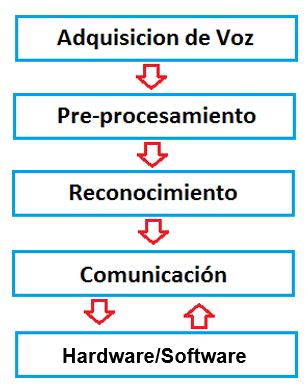
\includegraphics[width=0.25\textwidth]{Imagenes/Cap2/image004}
\end{center}
\begin{center}
\vskip -0.5cm
\caption{\small{Diagrama de bloques del proceso general del reconocimiento de voz.}}
\label{fig:figura2.4}
{\small{Fuente: \cite{rama}}}
\end{center}
\end{figure}

Existe una comunicación bilateral en aplicaciones en las que la interfaz de voz está íntimamente relacionada al resto de la aplicación. Estas pueden guiar al reconocedor especificando las palabras o estructuras que el sistema puede utilizar. Otros sistemas tienen una comunicación unilateral.
\vskip 0.5cm
Los procesos de preprocesamiento, reconocimiento y comunicación deberían ser invisibles al usuario de la interfaz. El usuario lo nota en el desempeño del sistema de manera indirecta como: certeza en el reconocimiento y velocidad. Estas características se utilizan para evaluar un sistema de reconocimiento de voz.
\vskip 0.5cm
Una vez visto el proceso general de un sistema de reconocimiento de voz, a continuación, veremos los módulos necesarios a detalle para el diseño y construcción de un sistema de reconocimiento de voz del locutor dependiente del texto. 
\vskip 0.5cm
Los diagramas de bloques que se muestran en las Figuras \ref{fig:figura2.5} y \ref{fig:figura2.6} ilustran, de forma general, los procesos que se realizan en el entrenamiento y reconocimiento de palabras aisladas, respectivamente.

\begin{figure}[ht]
\begin{center}
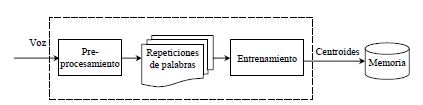
\includegraphics[width=0.55\textwidth]{Imagenes/Cap2/image005}
\end{center}
\begin{center}
\vskip -0.5cm
\caption{\small{Diagrama de bloques para la etapa de entrenamiento.}}
\label{fig:figura2.5}
{\small{Fuente: \cite{navarrete}}}
\end{center}
\end{figure}

\begin{figure}[ht]
\begin{center}
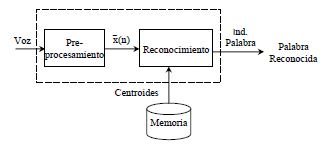
\includegraphics[width=0.5\textwidth]{Imagenes/Cap2/image006}
\end{center}
\begin{center}
\vskip -0.5cm
\caption{\small{Diagrama de bloques para la etapa de reconocimiento.}}
\label{fig:figura2.6}
{\small{Fuente: \cite{navarrete}}}
\end{center}
\end{figure}

Si observamos las Figuras \ref{fig:figura2.5} y \ref{fig:figura2.6}, existe un módulo común en ambas etapas, el preprocesamiento. Por esta razón, el preprocesamiento se manejará como un módulo independiente, para efecto del análisis.
\vskip 0.5cm
En la Figura \ref{fig:figura2.5}, durante la etapa de entrenamiento se capturan diferentes señales de voz, a la que denominaremos repeticiones de palabras. A cada repetición se le aplica preprocesamiento para obtener una palabra delimitada, después se agrupan todas las palabras recortadas y con ellas se obtienen sus centroides correspondientes, para luego ser guardados en memoria (base de datos).
\vskip 0.5cm
Como se observa en la Figura \ref{fig:figura2.6}, en la etapa de reconocimiento se captura la palabra que se desea reconocer. A esta palabra, también se le aplica preprocesamiento, para recortarla. Utilizando los centroides, calculados durante el entrenamiento y almacenados en la memoria, se realizan las comparaciones necesarias, para efectuar el reconocimiento. El éxito del evento dependerá de ciertos parámetros estadísticos obtenidos mediante el análisis de una población de resultados.

\subsection{Procesamiento o análisis de la señal de voz}
La finalidad del procesamiento de la señal de voz es obtener una representación más útil o conveniente de la información contenida en esta. Como se mostró anteriormente, la señal de voz es una composición compleja de sonidos, pero mediante un análisis, se puede mostrar que está formada por la combinación de componentes a diferentes frecuencias, producidas por la excitación periódica o aperiódica de las resonancias en el tracto vocal, principalmente entre 80 y 8000 Hz, \cite{rowden}.
\vskip 0.5cm
Las técnicas de análisis se pueden clasificar en dos categorías: en el dominio del tiempo o en el dominio de la frecuencia. Los procedimientos en el dominio del tiempo, se denominan así, porque éstos tienen que ver directamente con la señal de voz. El atractivo de estas representaciones es la facilidad con la que se pueden implementar, no obstante, estas suministran un medio útil para estimar otras características importantes de la señal. En contraste, los métodos en el dominio de la frecuencia involucran, ya sea de manera explícita o implícita, alguna forma de representación del espectro en frecuencia. 
\vskip 0.5cm
La mayoría de estas se basan en el modelo fuente-filtro, ver en \cite{rowden}, para la producción de la voz. Así que esencialmente, el análisis es el proceso en el cual, a partir de una señal de voz, se estiman los parámetros variantes en el tiempo del filtro, de tal manera que su objetivo principal es el estimar la respuesta en frecuencia del filtro que representa al tracto vocal. 
\vskip 0.5cm
A continuación, veremos los conceptos necesarios para la construcción de un reconocedor de voz, por cada una de las etapas que este tiene.

\subsubsection{Preprocesamiento}
En el preprocesamiento se recibe una señal de voz y se digitaliza determinando sus límites, esta señal puede contener ruido externo o no, si la tiene se aplicará un filtro de eliminación de ruido. Luego se le aplica un filtro de preénfasis, para realzar las frecuencias altas presentes en la voz. Después se la divide en tramas y a cada trama se le aplica una ventana para suavizar el espectro. 
\vskip 0.5cm
Es necesario aclarar que, cuando se inicializa el sistema, se determinan ciertos parámetros (umbrales) necesarios para la detección de inicio y fin de la señal de voz. Estos parámetros se calculan recolectando muestras del ruido presente en el ambiente circundante. El módulo encargado de realizar este proceso se denomina ruido ambiental. Finalmente, con las tramas provenientes del ventaneo y con los umbrales originados por el ruido ambiental, se determina el inicio y fin de la señal de voz, tal como se muestra en la Figura \ref{fig:figura2.7}.
\vskip 0.5cm
Como ya se mencionó, el preprocesamiento es un módulo presente en las etapas de entrenamiento y reconocimiento. Sin embargo, existe una diferencia sutil, durante el entrenamiento cada palabra recortada se almacena, y en un archivo independiente se determinan los centroides representativos de esta, mientras que en el reconocimiento se utiliza directamente el archivo con los centroides para hacer las comparaciones.

\begin{figure}[ht]
\begin{center}
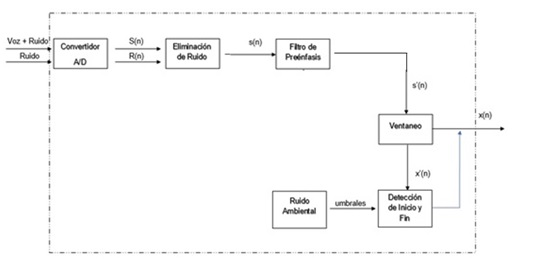
\includegraphics[width=0.83\textwidth]{Imagenes/Cap2/image007}
\end{center}
\begin{center}
\vskip -0.5cm
\caption{\small{Diagrama de bloques para el módulo de preprocesamiento.}}
\label{fig:figura2.7}
{\small{Fuente: Adaptación de \cite{navarrete}}}
\end{center}
\end{figure}

El preprocesamiento consta de los siguientes módulos: convertidor A/D, eliminación de ruido, filtro de preénfasis, ventaneo o segmentación, detección de ruido ambiental y detección de inicio y fin de la señal de voz. Estos módulos se describen a continuación:

\begin{enumerate}
\item[a)]Digitalización de la señal de voz
\par
Para poder manipular la señal de voz esta debe de ser transformada a una señal digital, así podrá ser utilizada por el software de programación, este proceso se lleva a cabo en etapas con consideraciones variables que hacen que la adquisición de la señal sea de forma correcta.

\newpage
\begin{figure}[ht]
\begin{center}
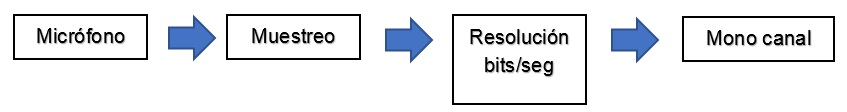
\includegraphics[width=0.6\textwidth]{Imagenes/Cap2/image008}
\end{center}
\begin{center}
\vskip -0.5cm
\caption{\small{Diagrama de la adquisición de voz.}}
\label{fig:figura2.8}
{\small{Fuente: \cite{eyra}}}
\end{center}
\end{figure}

\begin{enumerate}
\item[•]Obtención de información mediante un micrófono
\par
El micrófono es un transductor electroacústico. Su función es la de transformar la presión acústica ejercida sobre su capsula por las ondas sonoras en energía eléctrica.
\vskip 0.5cm
Como se dijo, el audio es un fenómeno analógico. Para grabar una señal de voz se hace la conversión de la señal analógica del micrófono en una señal digital por medio del conversor A/D en la tarjeta de sonido. Cuando un micrófono está operando las ondas de sonido hacen que vibre el elemento magnético del micrófono, causando una corriente eléctrica hacia la tarjeta de sonido, donde el conversor A/D básicamente graba los voltajes eléctricos en intervalos específicos.
\vskip 0.5cm
Hay dos factores importantes durante este proceso. Primero está la taza de muestreo, es decir que tan seguido los valores de voltaje son grabados. Segundo, son los bits por segundo, en otras palabras, que tan exactamente los valores son grabados. Un tercero podría ser el número de canales (mono o estéreo), pero para las aplicaciones de reconocimiento de voz un canal (mono) es suficiente.

\item[•]Ancho de banda y muestreo
\par
Según \cite{claudio}, el ancho de banda para las señales de voz es de aproximadamente unos 16000 Hz, pero la mayor parte de la energía se concentra en las frecuencias menores a 7000 Hz. No obstante, un ancho de banda de 3500 Hz es suficiente para poder entender el mensaje contenido en la señal de voz.
\vskip 0.5cm
El valor para la frecuencia de muestreo se determina mediante el teorema del muestreo de Nyquist, que establece que, si la componente en frecuencia más alta presente en la señal de voz es \textit{$f_{max}$}, entonces para poder reconstruir apropiadamente la señal a partir de las muestras obtenidas, la frecuencia de muestreo \textit{$f_{s}$} debe satisfacer lo siguiente:
\begin{center}
$f_{s} \geq 2f_{max}$ \hspace{1cm} $f_{N} \doteq f_{max}$ \hspace{1cm} $f_{s} \geq 2f_{N}$
\end{center}
En donde a $f_{N}$ se le conoce como la frecuencia de Nyquist. Por lo tanto, el periodo de muestreo $T_{s}$ es igual al inverso de la frecuencia de muestreo \textit{$f_{s}$}:
\begin{center}
$T_{s} \doteq \frac{1}{f_{s}}$
\end{center}
Si se emplea una frecuencia de muestreo menor que el doble de la frecuencia de Nyquist, entonces sucede un fenómeno conocido como \textit{aliasing}, para el cual una señal senoidal a cierta frecuencia pudiera parecer otra señal de menor frecuencia, como si esta fuera un alias de la original. Si ocurriera un aliasing en la señal de voz, se insertarían algunas componentes en frecuencia no deseadas que la distorsionarían.
\vskip 0.5cm
Puesto que el ancho de banda de una señal de voz se reduce durante la conversión A/D, para su procesamiento se suelen utilizar básicamente dos frecuencias de muestreo, la primera de \textit{$f_{s}$ = 16000 Hz} para obtener un ancho de banda o una frecuencia de Nyquist de \textit{$f_{N}$ = 8000 Hz}, y la segunda de \textit{$f_{s}$ = 8000 Hz} que corresponde a un ancho de banda o una frecuencia de Nyquist de \textit{$f_{N}$ = 4000 Hz}, \cite{herrera}.
\vskip 0.5cm
En cualquier caso, el muestreo periódico de una señal analógica de voz \textit{x(t)}, proporciona una representación de esa señal mediante una secuencia de muestras \textit{x(n)}, que se pueden obtener mediante la siguiente relación:
\begin{center}
$x(n) \doteq x(t) \textbf{|}_{t \doteq nT_{s}}$ \hspace{1cm} $n \doteq 0,1,2,3,...,N_{x} - 1$
\end{center}
En donde $N_{x}$ es el número total de muestras presentes en la señal de voz. La Figura \ref{fig:figura2.10} ilustra el muestreo de una señal analógica de voz a una frecuencia de muestreo de \textit{$f_{s}$ = 8000 Hz}, así que cada una de las \textit{$N_{x}$ = 21} muestras se toman cada \textit{$T_{s}$ = 0.125 ms}.

\begin{figure}[ht]
\begin{center}
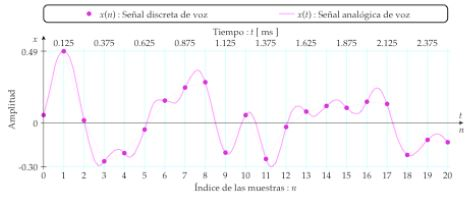
\includegraphics[width=0.65\textwidth]{Imagenes/Cap2/image010}
\end{center}
\begin{center}
\vskip -0.5cm
\caption{\small{Muestreo de una señal de voz.}}
\label{fig:figura2.10}
{\small{Fuente: \cite{herrera}}}
\end{center}
\end{figure}

La señal discreta de voz \textit{x(n)} esta indizada por la variable \textit{n}, que da una normalización de la señal, es decir, que ésta no contiene ninguna información explícita acerca de la frecuencia de muestreo. Aunque las muestras definen una señal discreta, se acostumbra unir éstas para que formen una curva continua para representar la señal de voz.

\item[•]Resolución o cuantificación
\par
La cuantificación es uno de los pasos que se siguen para lograr la digitalización de una señal analógica. Este proceso convierte una sucesión de muestras de amplitud continua en una sucesión de valores discretos preestablecidos según el código utilizado.
\vskip 0.5cm
Durante el proceso de cuantificación se mide el nivel de tensión de cada una de las muestras, obtenidas en el proceso de muestreo, y se les atribuye un valor finito de amplitud, seleccionado por aproximación dentro de un margen de niveles previamente fijado. En la Figura \ref{fig:figura2.11} se muestra un ejemplo utilizando 2 bits donde se pueden representar 4 valores diferentes y con 4 bits 16 valores.

\begin{figure}[ht]
\begin{center}
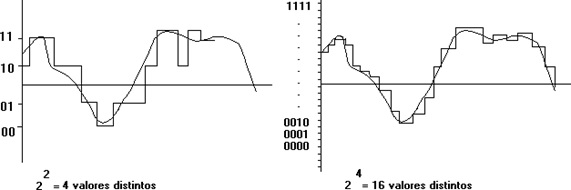
\includegraphics[width=0.6\textwidth]{Imagenes/Cap2/image011}
\end{center}
\begin{center}
\vskip -0.5cm
\caption{\small{Señal cuantificada con 2 y 4 bits respectivamente.}}
\label{fig:figura2.11}
{\small{Fuente: \cite{eyra}}}
\end{center}
\end{figure}

Esto se puede ver como la resolución:
\begin{enumerate}
\item[-]El error o diferencia entre la señal original y la reconstruida se percibe como ruido.
\item[-]Por lo tanto, a mayor resolución menor ruido como consecuencia.
\item[-]La resolución (número de bits por muestra) se describe generalmente en términos de la relación señal a ruido (Signal to Noise Ratio o SNR).
\item[-]A mayor SNR es mayor la fidelidad de la señal digitalizada.
\item[-]SNR es aproximadamente $2^B$ (B=bits/muestra)
\item[-]Es independiente de la frecuencia de muestreo.
\end{enumerate}
\vskip 0.3cm
Existen diferentes técnicas de cuantificación: uniforme, no uniforme, logarítmica y vectorial, \cite{rama}. En los cuantificadores uniformes o lineales la distancia entre los niveles de reconstrucción es siempre la misma, la mayoría usan un número de niveles que es una potencia de 2, ver Figura \ref{fig:figura2.12}. No hacen ninguna suposición acerca de la señal a cuantificar, de allí que no proporcionen los mejores resultados, pero su ventaja es que son más fáciles y económicos al implementarlos, es por esto que usaremos esta técnica para nuestra investigación.
\vskip 0.4cm
La cuantificación más usada, es de 8 bits, mínimo requerido para una calidad baja, puede mejorarse su SNR con una técnica no lineal de cuantificación, pero se obtienen excelentes resultados aumentando la cuantificación a 16 bits, \cite{kaifu}.
\begin{figure}[ht]
\begin{center}
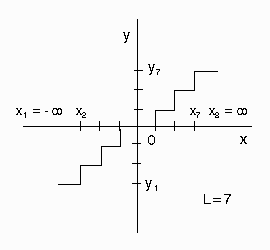
\includegraphics[width=0.3\textwidth]{Imagenes/Cap2/image012}
\end{center}
\begin{center}
\vskip -0.5cm
\caption{\small{Señal cuantificada uniformemente.}}
\label{fig:figura2.12}
{\small{Fuente: \cite{rama}}}
\end{center}
\end{figure}
\end{enumerate}

\item[b)]Eliminación de ruido y normalización
\par
El ruido es como una señal no deseada, es un elemento independiente de la señal, pero como consecuencia puede afectar la calidad de la misma. Para cancelar el ruido y mejorar la calidad se han desarrollado diversas técnicas de procesamiento de señal, dentro de los cuales se puede mencionar los filtros adaptativos, que es una técnica de las varias que existen hoy en día y es importante considerar los tipos de ruidos existentes en los canales de comunicación, \cite{henry}.

\begin{enumerate}
\item[-]Ruido aditivo: Se puede considerar todo aquel ruido procedente de distintas fuentes que coexistan en el mismo entorno acústico.
\item[-]Señales interferentes: En el caso de señales de voz, se considera señal interferente a toda aquella que proceda de otros locutores, que no sean objeto de interés.
\item[-]Reverberación: Producida por la propagación multitrayectoria que se dan en los entornos acústicos cerrados o semicerrados. No se trata exactamente de ruido, sino de una forma de distorsión.
\item[-]Eco: Producida generalmente por el acoplamiento entre los micrófonos y los altavoces. Igual que en el caso anterior se trata de una forma de distorsión.
\item[-]Diafonía: Sonido indeseado que se origina en el receptor, y es la consecuencia del acoplamiento de este canal con otro, permitiendo el paso de señales del mismo origen.
\end{enumerate}

\begin{enumerate}
\item[•]Cancelación de ruido aditivo
\par
En los sistemas de cancelación de ruido podemos encontrar dos tipos de filtros, los filtros digitales y los filtros adaptativos. Los filtros digitales solo pueden ser usados en ambientes de ruido estacionario, ya que es necesario conocer a priori las estadísticas del ruido, una solución a esto son los filtros adaptativos.
\vskip 0.5cm
El propósito de los filtros digitales es separar señales que se han combinado y restaurar señales que se han distorsionado de alguna manera. La separación de señales se requiere cuando una señal se ha contaminado con una interferencia, ruido, u otras señales. Los filtros Weiner y filtros Kalman son ejemplos de filtros digitales, ver la Figura \ref{fig:figura2.14}, \cite{shubhra}.

\newpage
\begin{figure}[ht]
\begin{center}
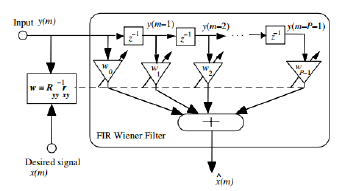
\includegraphics[width=0.5\textwidth]{Imagenes/Cap2/image014}
\end{center}
\begin{center}
\vskip -0.5cm
\caption{\small{Ilustración de la estructura de un filtro Wiener.}}
\label{fig:figura2.14}
{\small{Fuente: \cite{shubhra}}}
\end{center}
\end{figure}
\vskip -0.5cm
Por otro lado, los filtros adaptativos confian en el uso de una fuente de ruido para eliminar el ruido de una señal recibida. Básicamente, un cancelador de ruido adaptativo es un arreglo de doble entrada de lazo cerrado del sistema de realimentación como se ilustra en la Figura \ref{fig:figura2.15}, se derivan las dos entradas del sistema de un par de sensores: un sensor primario y un sensor de referencia (auxiliar), ver Figura \ref{fig:figura2.15}.

\begin{figure}[ht]
\begin{center}
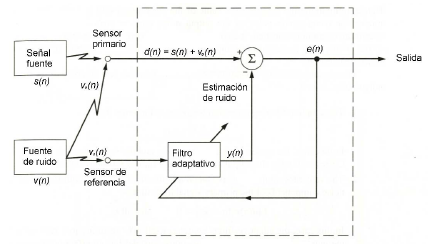
\includegraphics[width=0.65\textwidth]{Imagenes/Cap2/image015}
\end{center}
\begin{center}
\vskip -0.5cm
\caption{\small{Cancelador de ruido adaptativo.}}
\label{fig:figura2.15}
{\small{Fuente: \cite{walter}}}
\end{center}
\end{figure}

Específicamente, nosotros tenemos lo siguiente:
\begin{enumerate}
\item[1.]El sensor primario recibe una señal que lleva información \textit{s(n)} adulterada por un ruido aditivo \textit{$v_{0}(n)$}, como se muestra en la Ecuación \eqref{eq:ecuacion1}.
\vskip -1cm
\begin{equation}
\label{eq:ecuacion1}
d(n) = s(n) + v_{0}(n)
\end{equation}

La señal $s(n)$ y el ruido $v_{0}(n)$ están sin correlación una de la otra, esto es:
\vskip -1cm
\begin{equation}
\label{eq:ecuacion2}
E[s(n)v_{0}(n-k)] = 0 \hspace{1cm} \text{para todo \textit{k}}
\end{equation}

Donde $s(n)$ y $v_{0}(n)$ se suponen que son valores reales.

\item[2.]El sensor de referencia recibe un ruido $v_{1}(n)$ que no tiene correlación con la señal $s(n)$ pero si tiene correlación con el ruido $v_{0}(n)$, el cual es obtenido con el sensor primario junto a la señal que se desea recuperar; esto es:
\begin{equation}
\label{eq:ecuacion3}
E[s(n)v_{1}(n-k)] = 0 \hspace{1cm} \text{para todo \textit{k}}
\end{equation}
\vskip -1cm
\begin{equation}
\label{eq:ecuacion4}
E[v_{0}(n)v_{1}(n-k)] = p(k)
\end{equation}

Donde, la señal es un valor real y $p(k)$ es una correlación cruzada desconocida para el retardo $k$. La señal de referencia $v_{1}(n)$ es procesada por un filtro adaptativo para producir la salida:
\begin{equation}
\label{eq:ecuacion5}
y(n) = \sum_{k=0}^{M-1}\hat{w}_{k}(n)v_{1}(n-k)
\end{equation}

Donde, los $\hat{w}_{k}(n)$ son los valores de coeficientes (reales) ajustables del filtro adaptativo. La salida del filtro $y(n)$ es restada de la señal principal $d(n)$, conocida como la respuesta deseada para el filtro adaptativo. La señal de error se define por:
\begin{equation}
\label{eq:ecuacion6}
e(n) = d(n) - y(n)
\end{equation}

Así, sustituyendo la Ecuación \eqref{eq:ecuacion1} en la Ecuación \eqref{eq:ecuacion6}, se obtiene:
\begin{equation}
\label{eq:ecuacion7}
e(n) = s(n) + v_{0}(n) - y(n)
\end{equation}

La señal de error es la que se utiliza para ajustar los valores de coeficientes del filtro adaptativo y el lazo de control alrededor de las operaciones de filtrado y sustracción están relacionados. Note que la señal que lleva la información es cierta parte de la señal $e(n)$, como se indica en la Ecuación \eqref{eq:ecuacion7}.
\vskip 0.5cm
La señal de error $e(n)$ constituye la salida total del sistema. De la Ecuación \eqref{eq:ecuacion7} se puede ver, que la componente de ruido en la salida del sistema es $v_{0}(n) - y(n)$. Ahora comienza su labor el filtro adaptativo para minimizar el error cuadrático medio de la señal $e(n)$. La señal esencial $s(n)$ que lleva la información, no es afectada por el cancelador de ruido adaptativo.
\vskip 0.5cm
Así que, minimizando el error cuadrático medio de la señal $e(n)$ es equivalente a minimizar el error cuadrático medio del ruido de salida $v_{0}(n) - y(n)$. Con la señal $s(n)$ que permanece esencialmente constante, esto lleva a que la minimización del error cuadrático medio de la señal, es ciertamente la misma como la maximización de la razón señal a ruido de la salida del sistema.
\end{enumerate}
\vskip 0.5cm
El uso efectivo del cancelador de ruido adaptativo requiere que se coloque el sensor de referencia en el campo de ruido del sensor primario.
\vskip 0.5cm
\item[•]Estructura de los filtros adaptativos
\par
El algoritmo adaptativo debe disponer del error $e(n)$ para actualizar los coeficientes, ya que $e(n)$ permite definir las mejoras del filtro y determinar la forma en que han de modificarse dichos coeficientes. La eficiencia de un filtro adaptativo lineal depende de una serie de factores, como el tipo de filtro (IIR o FIR), la estructura del mismo (transversal, de celosía o sistólico), o la función de costo usada como criterio de adaptación (error cuadrático medio, mínimo error cuadrático, etc.).
\vskip 0.5cm
Nuestro estudio se va a centrar en el filtro FIR (Respuesta Finita al Impulso) por varias razones:
\begin{enumerate}
\item[-]El error cuadrático medio para un filtro transversal es una función cuadrática de los pesos del filtro. La superficie de error es un paraboloide con sólo un mínimo, y por ello, la búsqueda del error cuadrático medio mínimo es relativamente sencilla.
\item[-]Dado que los coeficientes del filtro son limitados, se puede controlar fácilmente la estabilidad del filtro.
\item[-]Existen algoritmos para la actualización de los coeficientes que con filtros FIR son mucho más simples y eficientes.
\item[-]Las prestaciones de estos algoritmos son perfectamente conocidas en términos de convergencia y estabilidad.
\end{enumerate}
De los tres tipos de estructuras de filtro que se distinguen en el contexto de un filtro adaptativo lineal, vamos a conceder toda la atención al tipo transversal.
\begin{figure}[ht]
\begin{center}
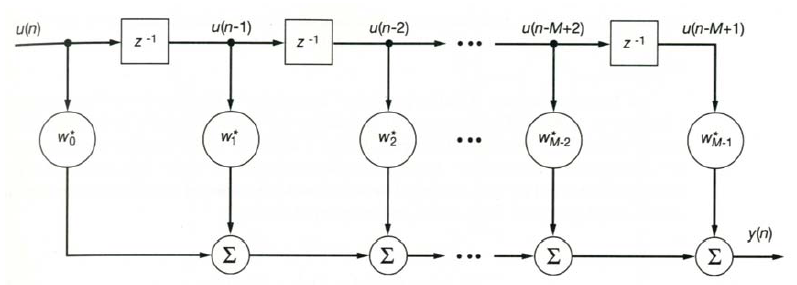
\includegraphics[width=0.6\textwidth]{Imagenes/Cap2/image016}
\end{center}
\begin{center}
\vskip -0.5cm
\caption{\small{Filtro transversal.}}
\label{fig:figura2.16}
{\small{Fuente: \cite{walter}}}
\end{center}
\end{figure}

Los filtros transversales, también llamados filtros directos de pesos retardados, consisten en tres elementos básicos, como se describió en la Figura \ref{fig:figura2.16}, primero los elementos de unidad de retardo, segundo el multiplicador, y tercero la sumatoria. El número de elementos de retardo usados en el filtro, mostrado como $M-1$ en la Figura \ref{fig:figura2.16}, determinan el filtro FIR, estos normalmente estan referidos al orden del filtro. Los elementos de retardo son identificados por el operador de la unidad de retraso $z^{-1}$. 
\vskip 0.5cm
En particular, cuando $z^{-1}$ opera en la entrada $u(n)$, la salida resultante es $u(n-1)$. El papel de cada multiplicador en el filtro es realizar el producto del valor de entrada por un coeficiente del filtro. Así un multiplicador conectado $k$ veces a entradas retardadas $u(n-k)$ produce la versión del escalar de que es el producto interno, $w^{*}_{k}u(n-k)$, donde $w_{k}$ va desde $k=1$ a $M$. El asterisco denota la conjugación compleja que asume la entrada y por consiguiente también los pesos actualizables son valores complejos. 
\vskip 0.5cm
El papel combinado de las sumatorias en el filtro es sumar los resultados de los productos individuales y producir una salida total del filtro. Para el filtro transversal descrito en la Figura \ref{fig:figura2.16}, la salida está dada de la siguiente manera:
\begin{equation}
\label{eq:ecuacion8}
y(n) = \sum_{k=0}^{M-1}W_{k} \cdot u(n-k)
\end{equation}
La ecuación es llamada sumatoria de convolución finita, en el sentido que la respuesta convoluciona el impulso de duración finita del filtro, $w^{*}_{n}$, con la entrada $u(n)$ del filtro, luego cada producto individual se suma para dar como resultado $y(n)$.
\vskip 0.5cm
La estructura transversal es la más sencilla de implementar, conduciendo a algoritmos igualmente sencillos. La estructura de celosía, presenta mejores propiedades, pues ofrece mayor robustez frente a errores de redondeo y una mayor eficiencia computacional. Sin embargo, aumenta la complejidad de los algoritmos. Por lo tanto, en el presente trabajo de tesis se adopta la primera estructura debido a su sencillez, pero aun así con buen desempeño.
\vskip 0.5cm
\item[•]Algoritmos de filtros adaptativos
\par
El filtro adaptativo ajusta sus coeficientes con un objetivo, garantizar la posible convergencia más rápida a los parámetros óptimos del punto de vista del criterio adoptado. La mayoría de algoritmos adaptivos significa modificaciones de los procedimientos iterativos normales para la solución del problema de minimización de la función de criterio en tiempo real. El más común de filtros adaptativos es el filtro transversal (escogido para nuestra investigación) y es usado por ejemplo en los algoritmos LMS (Mínimo Error Cuadrado Medio) y RLS (Mínimo Error Cuadrado Recursivo). Para lograr un buen desempeño del filtro adaptativo requiere el uso del mejor algoritmo adaptivo con baja complejidad computacional y un rango de convergencia rápido, es por esto que veremos el algoritmo LMS y su variante NLMS.

\begin{enumerate}
\item[-]Algoritmo Least Mean Square (LMS)
\par
Desarrollado por Windrow y Hoff, este algoritmo usa un descenso de la gradiente para estimar una variación del tiempo en la señal. El método de descenso de la gradiente encuentra un mínimo (si este existe), tomando los pasos en la dirección negativa de la gradiente y hace esto para ir ajustando los coeficientes del filtro para minimizar el error. La gradiente es un operador y se aplica para encontrar la divergencia de una función, que es el error con respecto en este caso al número de coeficientes. 
\vskip 0.5cm
El algoritmo LMS se ha aceptado por varios investigadores para la aplicación en el hardware debido a su estructura simple. Para llevarlo a cabo, las modificaciones tienen que ser hechas al algoritmo LMS original porque los bucles recursivos en la fórmula de actualización del filtro le impide ser un flujo lineal.
\vskip 0.5cm
La Ecuación \ref{eq:ecuacion9} muestra el detalle del algoritmo LMS, la evaluación de pesos:
\begin{equation}
\label{eq:ecuacion9}
w_{i}(n+1) = w_{i}(n) + \mu^{*}e(n)^{*}x(n-i)
\end{equation}
\vskip -0.5cm
Salida filtrada:
\vskip -0.5cm
\begin{equation}
\label{eq:ecuacion10}
y(n) = \sum_{k=0}^{M-1}w_{i}(n)^{*}x(n-i)
\end{equation}
\vskip 0.5cm
La estimación del error, donde $e(n)$ es la salida deseada:
\vskip -1cm
\begin{equation}
\label{eq:ecuacion11}
e(n) = d(n) - y(n)
\end{equation}

Donde la salida del filtro adaptivo $y(n)$ y el error de la señal $e(n)$ son obtenidos por las Ecuaciones \eqref{eq:ecuacion10} y \eqref{eq:ecuacion11}, respectivamente. En estas ecuaciones $x(n)$ es el vector de la señal de entrada, y $w(n)$ es el vector de pesos del filtro adaptivo. 
\vskip 0.5cm
De estas ecuaciones, en cada iteración la información de la mayoría de los recientes valores son requeridos y el procedimiento reiterativo se inicia con una suposición inicial $w_{0}$. El $\mu$ es el tamaño del paso de adaptación que depende del poder de la densidad espectral de la entrada de referencia $x(n)$ y $M-1$ es el orden del filtro y controla la estabilidad y velocidad de la convergencia del algoritmo LMS.
\vskip 0.5cm
\item[-]Algoritmo Normalized Least Mean Square (NLMS)
\par
La debilidad principal del LMS del tipo convencional radica en su complejidad seleccionando un valor conveniente para el parámetro de tamaño de paso que garantiza la estabilidad. Ante este inconveniente, fue propuesto el NLMS, controlando el factor de la convergencia del LMS a través de la modificación en un parámetro de tamaño de paso de tiempo variante. 
\vskip 0.5cm
El NLMS emplea un parámetro de tamaño de paso inconstante pensado a minimizar el error de salida instantáneamente el cual converge más rápidamente que el LMS convencional. El algoritmo LMS convencional experimenta en la gradiente problemas de amplificación de ruido cuando el factor de la convergencia $\mu$ es grande. La corrección se aplicó al vector de pesos $w(n)$ al $n+1$ de la iteración, es normalizada con respecto al cuadrado de la norma euclidiana del vector de entrada $x(n)$ a la iteración $n$. 
\vskip 0.5cm
Nosotros podemos expresar el algoritmo NLMS como un algoritmo de tamaño de paso de tiempo variante, calculando el factor de convergencia $\mu$ como en la Ecuación \eqref{eq:ecuacion12}.
\vskip -0.5cm
\begin{equation}
\label{eq:ecuacion12}
\mu(n) = \frac{\beta }{c+\left \| x(n) \right \|^{2}}
\end{equation}
\vskip 0.5cm
Dónde $\beta$ es la constante de adaptación del NLMS, que optimiza el rango de convergencia del algoritmo y debe satisfacer la condición $0< \beta <2$, y \textit{c} es el término constante para la normalización y siempre es menor que 1. Los pesos del filtro se actualizan por la Ecuación \eqref{eq:ecuacion13}
\vskip -0.5cm
\begin{equation}
\label{eq:ecuacion13}
w(n+1) = w(n) + \frac{\beta }{c+\left \| x(n) \right \|^{2}}e(n)x(n)
\end{equation}
\vskip 0.5cm
En comparación al LMS, el NLMS tiene tamaño de paso variante que hace al NLMS para converger más rápidamente. Para sacar mejores aplicaciones se han desarrollado varias variantes del LMS, ver la Tabla \ref{table:tabla24}.
\end{enumerate}
\vskip 0.5cm
Además del LMS, NLMS y sus variantes, existen otros algoritmos adaptivos como el algoritmo RLS (Mínimo Error Cuadrado Recursivo), el algoritmo CMA (Adaptivo de Módulo Constante), el algoritmo DMI (Adaptivo de Inversión de Matriz Directa), los cuales pueden verse en \citep{shubhra}.

\begin{center}
\begin{table}[h!]
\centering
\vskip -0.2cm
\caption{\small{Variantes del algoritmo LMS.}}
\label{table:tabla24}
\begin{tabular}{c}
\begin{minipage}{.9\textwidth}
\begin{center}
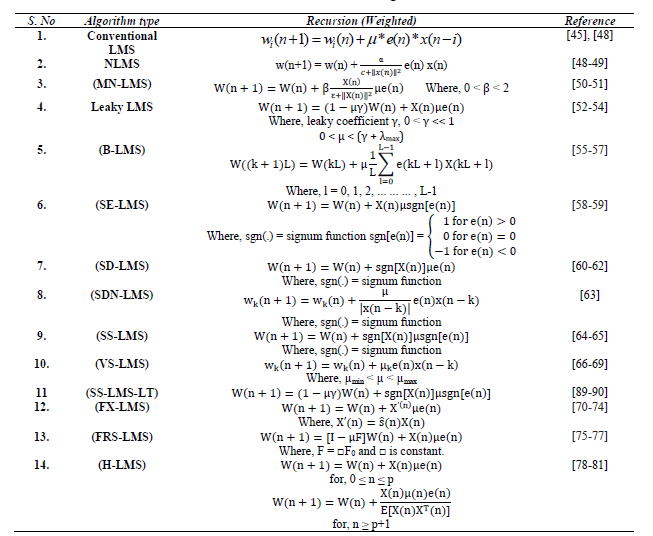
\includegraphics[width=0.7\textwidth]{Imagenes/Cap2/image019}
\end{center}
\end{minipage}
\end{tabular}
\begin{center}
\vskip 0.2cm
{\small{Fuente: \cite{shubhra}}}
\end{center}
\end{table}
\end{center}

\item[•]Convergencia
\par
Los coeficientes del filtro adaptativo se modifican constantemente hasta lograr que el error sea mínimo, es decir el algoritmo alcance la convergencia, dicho de otra manera, que la entrada se aproxime a la respuesta deseada. Para precisar lo que sucede, supongamos que el orden del filtro es $M=2$, es decir los coeficientes son de la forma $w(n)=[w1(n) w2(n)]$, siendo $\xi$ el error donde $\xi_{min}$ es el mínimo.
\vskip 0.5cm
Entonces el sistema se puede graficar en un espacio de tres dimensiones,ver la Figura \ref{fig:figura2.20}, cuando empieza el algoritmo, el error es grande y a medida que el tiempo transcurre, los coeficientes van descendiendo por la curva a una velocidad relativa a $\mu$ hasta llegar a $\xi_{min}$. Pero se debe tener en cuenta que este proceso no sucede de una manera trunca, sino similar a una pelota deslizándose por la pared interna cuando llega al fondo, pasa de largo y vuelve a subir, pero con menor impulso y luego vuelve a bajar y así sucesivamente hasta detenerse en el fondo. El tiempo que se demore en detenerse en el fondo es el tiempo de convergencia y $w_{0}$ es el punto de convergencia.

\begin{figure}[ht]
\begin{center}
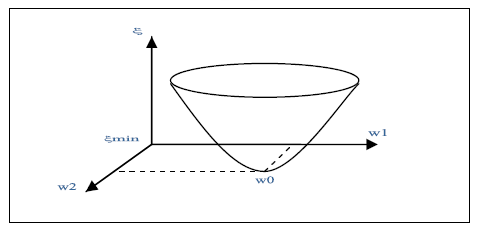
\includegraphics[width=0.4\textwidth]{Imagenes/Cap2/image020}
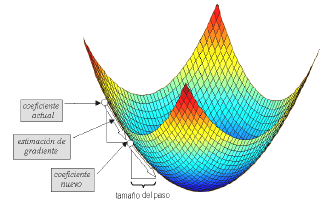
\includegraphics[width=0.4\textwidth]{Imagenes/Cap2/image021}
\end{center}
\begin{center}
\vskip -0.5cm
\caption{\small{Convergencia y error mínimo.}}
\label{fig:figura2.20}
{\small{Fuente: \cite{simon}}}
\end{center}
\end{figure}
\end{enumerate}
\vskip -0.5cm
En \citep{simon} se realizaron pruebas para obtener el mejor número de orden $M$ y tamaño de paso $\mu$ para el algoritmo LMS y el mejor número de orden $M$, la constante de adaptación $\beta$ y el término constante para la normalización $c$ para el algoritmo NLMS. Estas pruebas se realizaron con un micrófono primario ubicado a 2 metros de la fuente de ruido (equipo de sonido) y un segundo micrófono ubicado a 50 cm de esta fuente. Se concluyo que cuando se utiliza un tamaño de paso grande ($\mu > 0.03$) el error en un determinado momento se eleva, el valor de $W$ se torna inestable, por lo cual se debe elegir un valor menor. 
\vskip 0.5cm
En la Figura \ref{fig:figura2.21} se puede apreciar como la energía se va reduciendo desde $M=32$ hasta $M=128$, pero luego vuelve a incrementarse como se dijo anteriormente. Entonces se puede concluir que el mejor valor de $M$ bordea el valor 128.

\begin{figure}[ht]
\begin{center}
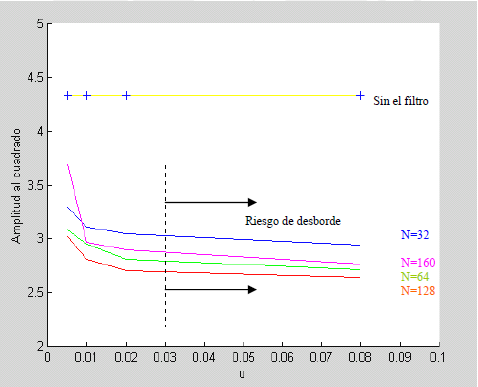
\includegraphics[width=0.45\textwidth]{Imagenes/Cap2/image022}
\end{center}
\begin{center}
\vskip -0.5cm
\caption{\small{Cuadrado promedio para diferentes valores de M y $\mu$ para el LMS.}}
\label{fig:figura2.21}
{\small{Fuente: \cite{simon}}}
\end{center}
\end{figure}
\vskip -0.5cm
El error varía poco para un tamaño de paso entre 0.02 y 0.08 además debe ser menor a 0.03 para evitar el desborde, por lo que se eligió el valor de 0.02 que asegura la estabilidad del filtro y mantiene el error a un nivel aceptable, ver la Figura \ref{fig:figura2.22}.

En la Figura \ref{fig:figura2.23} se puede apreciar que se obtuvo una buena eficiencia hasta 81dBC de ruido a 2m de distancia de los parlantes. Para el algoritmo NLMS se propuso los valores de $M =128$ al igual que el del LMS, con $\beta = 0.25$ y $c = 0.0001$.

\newpage
\begin{figure}[ht]
\begin{center}
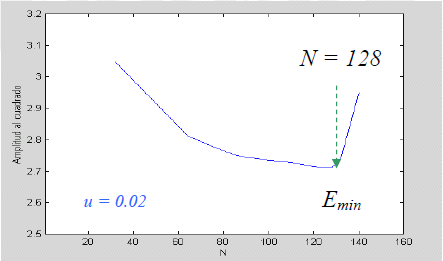
\includegraphics[width=0.45\textwidth]{Imagenes/Cap2/image023}
\end{center}
\begin{center}
\vskip -0.5cm
\caption{\small{Valor para el número de orden M con $\mu$\protect=0.02.}}
\label{fig:figura2.22}

{\small{Fuente: \cite{simon}}}
\end{center}
\end{figure}
\begin{figure}[ht]
\begin{center}
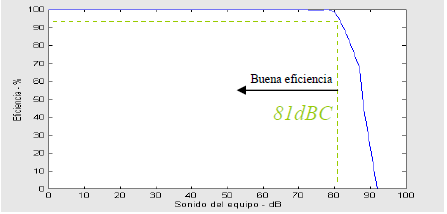
\includegraphics[width=0.5\textwidth]{Imagenes/Cap2/image024}
\end{center}
\begin{center}
\vskip -0.5cm
\caption{\small{Curva de eficiencia vs. sonido del equipo.}}
\label{fig:figura2.23}
{\small{Fuente: \cite{simon}}}
\end{center}
\end{figure}

Finalmente, esta etapa de eliminación de ruido estará conformada por dos submódulos, el primero será la eliminación de ruido donde evaluaremos los algoritmos LMS Y NLMS para luego elegir el que tenga un mejor desempeño y el segundo es la normalización de la señal después de haber aplicado el filtro adaptativo, debido a que puede haber un aumento en el espectro de potencia.

\newpage
En \cite{mathematics} se muestra la formula para la normalización de la señal:\\
$[c, d]$ = rango de entrada mínimo y máximo.\\
$[m, n]$ = rango de salida mínimo y máximo.\\
Donde:
\begin{equation}
\label{eq:ecuacion14}
A = (m-n)/(c-d)
\end{equation}
\vskip -1cm
\begin{equation}
\label{eq:ecuacion15}
B = m - A*c
\end{equation}

Entonces para la señal de entrada $E(n)$ obtenemos la salida normalizada $S(n)$:
\begin{equation}
\label{eq:ecuacion16}
S(n) = A^{*}E(n) + B
\end{equation}

\item[c)]Detección de inicio y fin de la señal de voz
\par
El problema de la localización del inicio y final de una muestra de voz en un fondo acústico de silencio es de vital importancia en muchas áreas del procesamiento de voz. El poder determinar cuál es el inicio y el final de una palabra proporciona ciertas ventajas como, procesar menor cantidad de información, comparar únicamente los patrones de información y evitar confusiones a causa del ruido o señales de fondo.
\vskip 0.5cm
La tarea de separar la voz del espacio de silencio no es una tarea tan simple como puede parecer, esto puede suceder sólo en ambientes acústicos con tasa extremadamente alta de señal a ruido, por ejemplo, las cámaras a prueba de eco o de ruido, donde son hechas las grabaciones de alta calidad. Para dichos ambientes con alta relación señal a ruido, la energía de los sonidos de voz de más bajo nivel (fricativos débiles) excede la energía del ruido del fondo, por ende, una simple medición de la energía es suficiente para realizar las mediciones. 
\vskip 0.5cm
Sin embargo, dichas condiciones ideales de grabación no son prácticas para las aplicaciones del mundo real. Por ende, la simple medición de la energía se convierte en una condición necesaria más no suficiente para separar los fricativos débiles del fondo de silencio.
\vskip 0.5cm
Algunos de los problemas que se presentan en la detección son:
\begin{enumerate}
\item[-]Silencios contenidos dentro de las palabras que tienen fonemas plosivos (\textit{ej. /t/, /p/, /k/}) que pueden confundirse con un falso principio o fin. 
\item[-]Presencia de espurias de ruido que se pueden confundir con la señal. 
\item[-]Los fonemas fricativos (\textit{ej. /f/, /th/, /h/, etc.}), ya que tienen baja energía.
\item[-]Sonidos cortos (\textit{ej. /t/, /p/, /k/}).
\item[-]Detección de fonemas nasales al final de la palabra.
\item[-]Respiraciones del locutor, que pueden confundirse por su duración.
\item[-]Los micrófonos tienen resonancia después de pronunciar una palabra (sobre todo en vocales).
\item[-]Los niveles de ruido pueden confundirse con la señal de voz.
\end{enumerate}

En este trabajo de tesis se evaluará el algoritmo por función de energía y los algoritmos propuestos por Rabiner y Sambur, la expuesta en \citep{unam} la denominaremos \textit{Tipo 1} y la de \citep{rabiner} la denominaremos \textit{Tipo 2}, para la localización de los puntos de inicio y final de la señal de voz de una grabación. El algoritmo de Rabiner y Sambur es muy útil y funciona muy bien en ambientes con una relación señal a ruido de al menos 30 dBC y está basado en dos mediciones de la voz, la energía de tiempo corto y la tasa de cruces por cero. Por último, se escogerá el que tenga mejor desempeño.

\begin{enumerate}
\item[•]Algoritmo por función de energía
\par
La señal digitalizada es escaneada y las zonas de silencio son removidas por medio del cálculo de energía en corto tiempo. En segmentos de 10 ms si la energía promedio es menor que un valor umbral, generalmente de valor 0.2 (proporcional a la energía promedio de la señal entera) es descartado, \cite{genoveva}. A continuación, se muestran las fórmulas que se utilizarán:

\begin{equation}
\label{eq:ecuacion17}
E_{n} = \sum_{m=0}^{N-1}\left | x[m] \right |^{2}
\end{equation}
\vskip -0.5cm
\begin{equation}
\label{eq:ecuacion18}
E_{avg} = \frac{1}{N}\sum_{k=1}^{N}\left | x[k] \right |^{2}
\end{equation}

Donde $E_{n}$ es la energía promedio de cada segmento y $E_{avg}$ es la energía promedio de la señal entera.

\item[•]Algoritmo de Rabiner y Sambur tipo 1
\par
Tanto la energía como la magnitud son útiles para distinguir segmentos sordos y sonoros en la señal de voz. Pero existen otras maneras para identificar segmentos sonoros, hay un método denominado \textit{cruces por cero y máximos}, se puede decir que una señal clasificada como ruido (la \textit{s} es un ruido de alta frecuencia) provoca en la amplitud un cambio de signo, de esta manera se pueden localizar consonantes fricativas.
\vskip 0.5cm
El algoritmo de Rabiner y Sambur combina la energía instantánea en una trama, con medidas de tasas de cruce por cero y confían en que un nivel alto de energía es el mejor estímulo para la detección. Se asume que la tasa de cruces por cero es bien distinta en zonas de voz con baja energía o de ruido de fondo y seria el punto adicional para determinar los límites de la voz.

\begin{enumerate}
\item[-]Energía de tiempo corto
\par
La energía de la voz $E(n)$, se define como la suma de las magnitudes de la voz al cuadrado en intervalos centrados de 10 ms, todo medido sobre el intervalo de medición, tal como se definió en la Ecuación \eqref{eq:ecuacion17}.
\vskip 0.5cm
En donde, $x(n)$ son las muestras de voz muestreadas a la frecuencia escogida. El escoger una ventana de 10 ms para el cálculo de la energía y el uso de la función de magnitud en lugar del cuadrado de la magnitud, se realizó porque puede causar un aumento en el espectro de la potencia, además así podemos aumentar la velocidad de computo, debido a que requerirá de una operación menos. La función de magnitud se define en la Ecuación \eqref{eq:ecuacion22}.

\item[-]Tasa de cruces por cero
\par
La tasa de cruces por cero de una grabación de voz $Z(n)$ se define como el número de cruces por cero en un intervalo de 10 ms. Aunque esta es altamente susceptible a ruido de 60 Hz, en la mayoría de los casos es una medida muy buena y razonable de la presencia o ausencia de silencio en la grabación.
\vskip 0.5cm
La principal suposición que se realiza al momento de aplicar este algoritmo es que los primeros 100 ms de grabación son silencio. Es por eso que, en este intervalo de tiempo, las estadísticas de silencio en el fondo de la grabación son medidas. Estas mediciones incluyen, la media de los valores de los datos digitalizados y la desviación estándar de la tasa de cruces por cero, así como la energía promedio.
\begin{equation}
\label{eq:ecuacion19}
Z(n) = \sum_{m=-\infty}^{\infty}\left | [x(m)] - [x(m-1)] \right |r(n-m)
\end{equation}
Donde:
\begin{equation}
\label{eq:ecuacion20}
\begin{split}
x(n)&= 1, x(n) \geq 0 \\ 
 &= -1, s(n) < 0
\end{split}
\end{equation}
Y
\begin{equation}
\label{eq:ecuacion21}
\begin{split}
r(n)&= \frac{1}{2N}, 0 \leq n \leq N-1 \\
 &= 0, \text{de otra manera}
\end{split}
\end{equation}
\vskip 0.2cm
\item[-]Algoritmo para la detección de inicio
\par
\begin{enumerate}
\item[1.]Por cada trama de 128 muestras, calcular las funciones: magnitud promedio $M_{n}$ y cruce por ceros $Z_{n}$, partiendo de las ecuaciones \eqref{eq:ecuacion17}, \eqref{eq:ecuacion19}, \eqref{eq:ecuacion20}, \eqref{eq:ecuacion21} estas funciones se definen a continuación: 
\begin{equation}
\label{eq:ecuacion22}
M_{n} = \sum_{m=0}^{N-1}\left | x[m] \right |
\end{equation}

\begin{equation}
\label{eq:ecuacion23}
Z_{n} = \frac{\sum\limits_{m=0}^{N-2}\left | sign(x[m+1]) - sign(x[m]) \right |}{2N}
\end{equation}
\item[2.]Para obtener las estadísticas del ruido ambiental se considera que las primeras diez ventanas son ruido, con lo cual se tiene:
\begin{equation}
\label{eq:ecuacion24}
\begin{split}
Ms_{n} &= \{M_{1},M_{2},...,M_{10}\}\\ 
Zs_{n} &= \{Z_{1},Z_{2},...,Z_{10}\}
\end{split}
\end{equation}
Donde $Ms_{n}$ es la magnitud del ruido y $Zs_{n}$ son los cruces por cero del ruido.
\item[3.]Calcular la media y la desviación estándar para las características del ruido y obtener los siguientes umbrales:
\begin{center}
\begin{table}[h!]
\centering
\caption{\small{Umbrales para la detección de inicio y fin de la señal de voz.}}
\label{table:tabla2.3}
\vskip 0.2cm
\begin{tabular}{|c|c|c|c|}
\hline
{\small\textbf{Umbral}} & {\small\textbf{Nombre del umbral}} & {\small\textbf{Valor}}  \\ 
\hline 
{\small $UmbSupEnrg$} & {\small Umbral Superior de Energía} & {\small $0.5^{*}max\{M_{n}\}$}  \\ 
\hline 
{\small $UmbInfEnrg$} & {\small Umbral Inferior de Energía} & {\small $\mu_{Ms} + 2^{*}\sigma_{Ms}$}  \\ 
\hline 
{\small $UmbCruCero$} & {\small Umbral de cruces por cero} & {\small $\mu_{Zs} + 2^{*}\sigma_{Zs}$}  \\ 
\hline
\end{tabular} 
\begin{center}
\vskip 0.2cm
{\small{Fuente: \cite{unam}}}
\end{center}
\end{table}
\end{center}

\vskip -1cm
\begin{equation}
\label{eq:ecuacion25}
\mu = \frac{\sum_{i}^{n}x_{i}}{N}
\end{equation}
\vskip -0.5cm
\begin{equation}
\label{eq:ecuacion26}
\sigma = \sqrt{\frac{\sum_{i}^{n}(x_{i} - \mu)^{2}}{N-1}}
\end{equation}
\vskip 0.5cm
Para el caso de $UmbSupEnrg$ se usa $M_{n}$ de la señal de voz (se considera a partir de las 10 tramas en adelante como señal de voz). En los siguientes dos casos, se usan los diez valores del ruido, obtenidos en el punto 2 para cada umbral. Recordar que es la media y la desviación estándar de la magnitud del ruido, así como la media y la desviación estándar del cruce por ceros del ruido.
\item[4.]Recorrer la función $M_{n}$ incrementando en una unidad a $n$ de 11 hasta que $M_{n} > UmbSupEnrg$. En este punto estamos garantizando presencia de señal. A este punto lo marcaremos como $I_{n}$.

\item[5.]Resulta lógico pensar que el inicio de la señal se encuentra en algún punto anterior a $I_{n}$, por lo que ahora recorremos la función $M_{n}$ desde $n = I_{n}$ hasta que $M_{n} < UmbInfEnrg$. Este punto lo marcaremos como $I_{e}$ y lo reconocemos tentativamente como el inicio de la señal.

\item[6.]Ahora disminuimos $n$, desde $n = I_{e}$ hasta $n = I_{e} \text{–} 25$ o en su defecto $n = 11$, verificando si se presenta alguna de las siguientes condiciones en la función de cruces por cero, ya que lo que ahora buscamos es la posibilidad de que un sonido no sonoro preceda a un sonido sonoro. Sí $Z_{n} < UmbCruCero$ significa que no encontramos alguna porción de la señal con aumento importante de frecuencia en 25 ventanas anteriores, por lo tanto, el inicio es $I_{e}$. Sí encontramos que $Z_{n} > UmbCruCero$ menos de tres veces seguidas significa que solo fue una espiga de ruido, el punto de inicio sigue siendo $I_{e}$.

\item[7.]Si encontramos que $Z_{n} > UmbCruCero$ al menos tres veces seguidas hemos encontrado un sonido no sonoro, entonces buscamos el punto $n$ para el cual $Z_{n} > UmbCruCero$ la primera de las más de tres veces, es decir, el punto para el cual la función $Z_{n}$ sobrepasa el umbral, indicando el comienzo del sonido no sonoro y desplazamos el inicio de la palabra de $I_{e}$ a $I_{z}$.
\end{enumerate}
\item[-]Algoritmo para la detección de fin
\par
Para la detección de fin de la señal de voz hacemos lo mismo, pero en sentido inverso a partir del punto (4) de la sección anterior, como si detectáramos un inicio con la señal invertida en el tiempo.
\end{enumerate}

\item[•]Algoritmo de Rabiner y Sambur tipo 2
\par
Al igual que el algoritmo anterior esta variante del algoritmo de Rabiner y Sambur también utiliza la energía de tiempo corto y la tasa de cruces por cero. La Figura \ref{fig:figura2.25} explica su funcionamiento, donde la señal se filtra en un ancho de banda entre 100 Hz y 4 KHz, con una frecuencia de muestreo de 10 KHz. De forma simple, el algoritmo de detección se basa en medidas de la energía cada 10 milisegundos.

\begin{figure}[ht]
\begin{center}
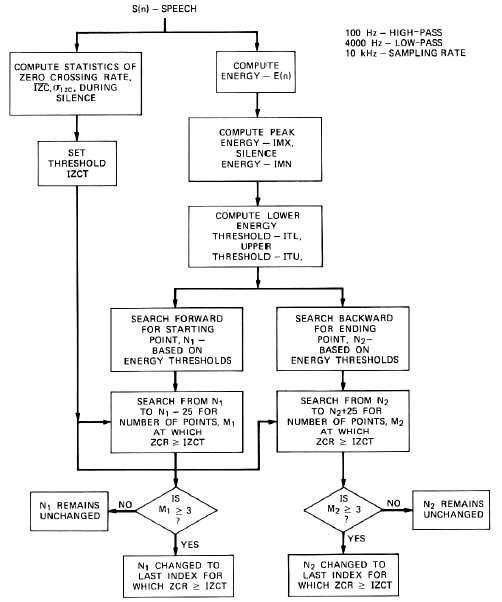
\includegraphics[width=0.55\textwidth]{Imagenes/Cap2/image026}
\end{center}
\begin{center}
\vskip -0.5cm
\caption{\small{Diagrama de flujo del algoritmo Rabiner y Sambur.}}
\label{fig:figura2.25}
{\small{Fuente: \cite{rabiner}}}
\end{center}
\end{figure}

Por otro lado, la tasa de cruces por cero $Z(n)$, también se calcula una vez cada trama de 10 milisegundos. El algoritmo supone que durante los 100 milisegundos primeros de la grabación no hay voz presente. Durante este periodo de silencio inicial se miden, la media $IZC$ (Cruce por Cero Integrado), y la desviación estándar \textit{IZC}, de la tasa de cruces por cero, la $IMX$ (Energía Máxima de Voz) y la $IMN$ (Energía Media del Ruido de fondo). Una vez obtenida la energía de toda la grabación se establecen los siguientes umbrales:

\begin{equation}
\label{eq:ecuacion27}
IZCT = MIN(IF,\overline{IZC} + 2\sigma _{IZC})
\end{equation}
\vskip -1.5cm
\begin{equation}
\label{eq:ecuacion28}
I1 = 0.03\cdot(IMX-IMN) + IMN
\end{equation}
\vskip -1.5cm
\begin{equation}
\label{eq:ecuacion29}
I2 = 4 \cdot IMN
\end{equation}
\vskip -1.5cm
\begin{equation}
\label{eq:ecuacion30}
ITL = MIN(I1,I2)
\end{equation}
\vskip -1.5cm
\begin{equation}
\label{eq:ecuacion31}
ITU = 5 \cdot ITL
\end{equation}

El umbral $IZCT$ tiene en cuenta el mínimo entre la tasa de cruces por cero promedios en una zona de silencio ($IZC$) más dos veces su desviación estándar y un umbral de tasa de cruces por cero $IF$, típicamente con valor 25. $I1$ simboliza la suma entre la $IMN$ (Energía Media del Ruido de fondo) y el 3\% de la diferencia entre el $IMX$ (\textit{Valor Máximo de la Energía de voz}) y la $IMN$ (Energía Media del Ruido de fondo). $I2$ es cuatro veces la $IMN$, $ITL$ el mínimo entre $I1$ e $I2$, y finalmente $ITU$, cinco veces $ITL$.
\vskip 0.5cm
En el detector sencillo que proponen Rabiner y Sambur, la decisión viene dada en función de una combinación de umbrales de energía y de tasa de cruces por cero. El diagrama de energía se puede visualizar en la Figura \ref{fig:figura2.26}.

\begin{figure}[ht]
\begin{center}
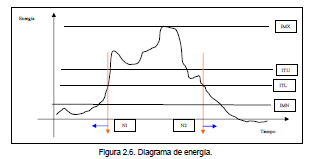
\includegraphics[width=0.55\textwidth]{Imagenes/Cap2/image027}
\end{center}
\begin{center}
\vskip -0.5cm
\caption{\small{Diagrama de energía.}}
\label{fig:figura2.26}
{\small{Fuente: \cite{varela}}}
\end{center}
\end{figure}

En este caso $IF$ es una constante de valor 25, ajustada manualmente, e $IMX$ es el pico de energía de la grabación incluyendo la voz principal. El comienzo del pulso, trama $N_{1}$, es el punto en el que la energía excede $ITL$:

\begin{enumerate}
\item[-]Si se supera $ITL$, estamos ante un posible pulso, pero todavía no se da ninguna confirmación debido a que podemos estar ante un pulso espurio.
\item[-]Una vez superado $ITL$, si además se supera $ITU$, ya se da la confirmación de pulso y se confirma también inicio de palabra. Se toma como inicio de pulso el instante de tiempo $N_{1}$ en el que supera $ITL$. Algo análogo ocurre con el final de pulso $N_{2}$.
\end{enumerate}

\newpage
\begin{figure}[ht]
\begin{center}
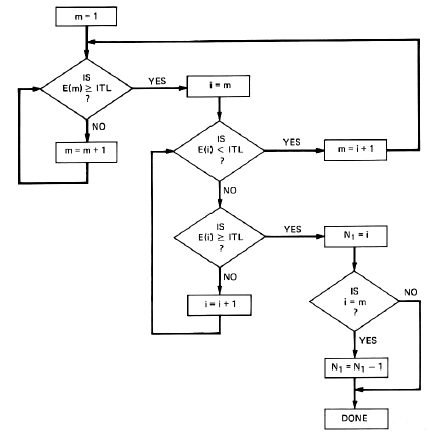
\includegraphics[width=0.35\textwidth]{Imagenes/Cap2/image028}
\end{center}
\begin{center}
\vskip -0.5cm
\caption{\small{Diagrama de flujo para la búsqueda del punto de inicio basado en la energía.}}
\label{fig:figura2.27}
{\small{Fuente: \cite{rabiner}}}
\end{center}

\begin{center}
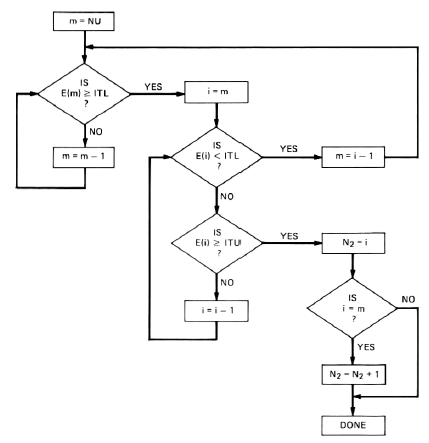
\includegraphics[width=0.35\textwidth]{Imagenes/Cap2/image029}
\end{center}
\begin{center}
\vskip -0.5cm
\caption{\small{Diagrama de flujo para la búsqueda del punto de fin basado en la energía.}}
\label{fig:figura2.28}
{\small{Fuente: \cite{rabiner}}}
\end{center}
\end{figure}

\newpage
Estos extremos son conservativos y se refina la localización de los extremos con la tasa de cruces por cero. El algoritmo examina desde $N_{1}$ hasta $N_{1}$ - $25$ y si el número de veces que se excede el umbral $IZCT$ es tres o más, el punto de comienzo se retrasa al primer punto (en el tiempo) en el que excede el mencionado umbral. De lo contrario, el comienzo se mantiene en $N_{1}$. De igual manera se opera en el intervalo comprendido entre $N_{2}$ y $N_{2} + 25$, ver Figura \ref{fig:figura2.29}.
\vskip 0.2cm
\begin{figure}[ht]
\begin{center}
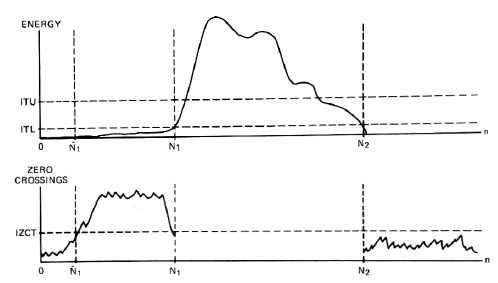
\includegraphics[width=0.45\textwidth]{Imagenes/Cap2/image030}
\end{center}
\begin{center}
\vskip -0.5cm
\caption{\small{Puntos de inicio y fin de la señal de voz.}}
\label{fig:figura2.29}
{\small{Fuente: \cite{rabiner}}}
\end{center}
\end{figure}
\end{enumerate}

\item[d)]Filtro de preénfasis
\par
Consiste en aplicar un filtro digital pasa altas de primer orden a la señal. Las frecuencias altas de los formantes se enfatizan por dos razones, primero para que no se pierda información durante la segmentación, ya que la mayoría de la información está contenida en las frecuencias bajas, y segundo para remover la componente DC de la señal, aplanándola espectralmente, \cite{stephen}.
\vskip 0.5cm
Las componentes de alta frecuencia presentes en la señal de voz, normalmente tienen una amplitud menor con respecto a las de baja frecuencia, debido a la atenuación que ocurre durante el mecanismo de producción de la voz, por lo que se necesita realizar un preénfasis, a fin de obtener una amplitud similar para todas las componentes, de tal manera que el espectro de la señal sea lo más plano posible. Este filtro FIR paso altas de primer orden, se encuentra definido por la siguiente ecuación, siendo $x(n)$ la señal de voz digitalizada:
\begin{equation}
\label{eq:ecuacion32}
x_{p} = x(n) - ax(n-1)\qquad
\begin{aligned}
& 0.9 \leq a \leq 1 \\
& n = 0,1,2,3,...,N_{x} - 1
\end{aligned}
\end{equation}
Donde $x_{p}(n)$ es la respuesta del filtro o la señal de voz con preénfasis y $\alpha$ es el parámetro de preénfasis. El valor más común para el parámetro de preénfasis es $\alpha = 0.95$, el cual proporciona un incremento de unos 20 dBC de amplificación para las componentes de alta frecuencia del espectro. No obstante, el valor exacto de este parámetro no es tan crítico. La Figura \ref{fig:figura2.31} muestra la magnitud de la respuesta en frecuencia de un filtro de preénfasis para una frecuencia de muestreo de $f_{s} = 8000 Hz$ y un parámetro de preénfasis $\alpha = 0.95$.

\begin{figure}[ht]
\begin{center}
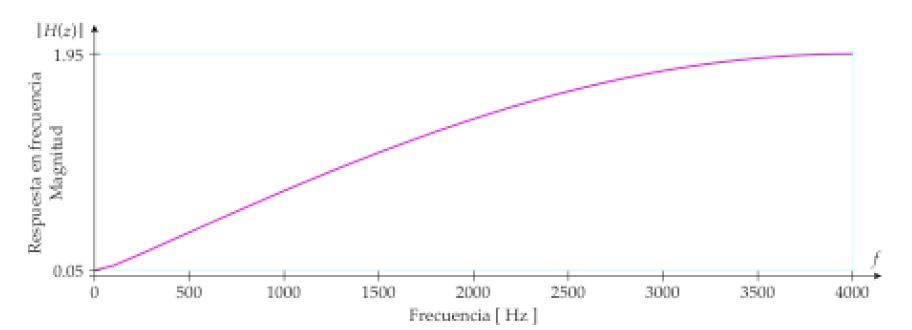
\includegraphics[width=0.56\textwidth]{Imagenes/Cap2/image032}
\end{center}
\begin{center}
\vskip -0.5cm
\caption{\small{Magnitud de la respuesta en frecuencia del filtro de preénfasis.}}
\label{fig:figura2.31}
{\small{Fuente: \cite{eyra}}}
\end{center}
\end{figure}

\item[e)]Segmentación
\par
Los métodos tradicionales de análisis en frecuencia son bastante confiables para las señales estacionarias, pero este no es el caso de la señal de voz. Entonces, para poder emplear estas técnicas, resulta necesario dividir la señal en segmentos cortos o tramas para poder realizar un análisis en tiempo corto. Estas tramas pueden ser separadas y procesadas de manera individual, como si fueran segmentos cortos de un sonido sostenido con propiedades fijas. Este proceso se repite tantas veces como sea necesario hasta que se haya abarcado completamente la señal.
\vskip 0.5cm
Estos segmentos o tramas de análisis, son de longitud finita, consisten de $N$ muestras y normalmente se traslapan entre sí, teniendo $S$ muestras de desplazamiento o separación entre el inicio de una trama y la siguiente:
\begin{equation}
\label{eq:ecuacion33}
x_{l} = x(n + l \cdot S)\qquad
\begin{aligned}
& l = 0,1,2,3,...,L-1 \\
& n = 0,1,2,3,...,N-1
\end{aligned}
\end{equation}
En donde $x_{l}(n)$ es la l-ésima trama y $L$ es la cantidad o el número total de tramas presentes en la señal de voz $x(n)$. La Figura \ref{fig:figura2.33} ilustra la división en tramas con traslape de una señal de voz, para una separación entre tramas de $S = N/3$ muestras.
\newpage
\begin{figure}[ht]
\begin{center}
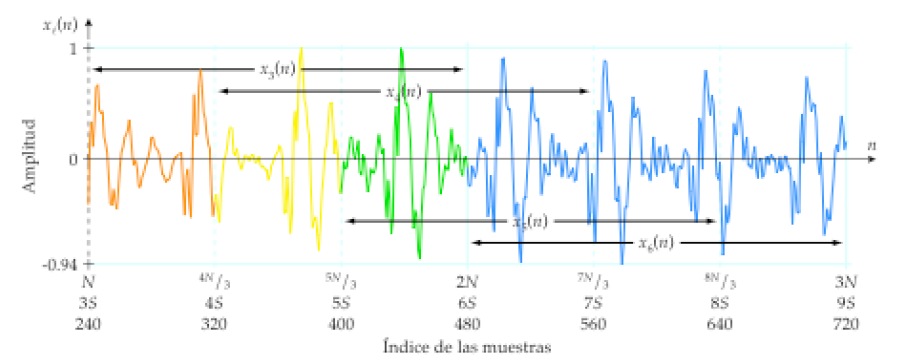
\includegraphics[width=0.75\textwidth]{Imagenes/Cap2/image034}
\end{center}
\begin{center}
\vskip -0.5cm
\caption{\small{División en tramas con traslape de una señal de voz.}}
\label{fig:figura2.33}
{\small{Fuente: \cite{eyra}}}
\end{center}
\end{figure}

A partir de la figura anterior, se puede observar que la cantidad o el número total de tramas en la señal de voz es $L$, se puede calcular mediante la siguiente ecuación:
\begin{equation}
\label{eq:ecuacion34}
L = \frac{N_{x} - N}{S} + 1
\end{equation}
Si $N>S$, entonces sí ocurre el traslape y $N \text{-} S$ muestras al final de las tramas son duplicadas al inicio de la siguiente trama. Entre mayor sea el traslape, la correlación entre las tramas adyacentes también será mayor y los cambios serán más suaves. Por otra parte, si $N < S$, entonces no hay traslape, pero además algunas porciones de la señal de voz se perderán, ya que no aparecerán en ninguna de las tramas. Por lo tanto, esta última situación resulta inaceptable en cualquier tipo de procesamiento de voz.
\vskip 0.5cm
Entonces, la señal de voz se divide en $L$ tramas para su análisis. Cada una de éstas se compone por $N$ muestras con $S$ muestras de separación entre tramas adyacentes. Sin embargo, para no perder las propiedades dinámicas o variantes en el tiempo de la señal de voz, es necesario volver a calcular otros coeficientes para la siguiente trama, para ello se recomienda aplicarle un ponderado a través de una ventana. Primero demos un vistazo a la más simple de las ventanas, la cual tiene una forma rectangular y se define como:
\begin{equation}
\label{eq:ecuacion35}
%
w(n) = 
\begin{cases}
0 & \text{para $n < 0$} \\ 
1 & \text{para $0 \leq  n \leq  N-1$} \\ 
0 & \text{para $n > N-1$} 
\end{cases}
%
\end{equation}
Esta ventana rectangular se usa de manera implícita cuando se extrae una trama de $N$ muestras a partir de una señal de voz:

\begin{figure}[ht]
\begin{center}
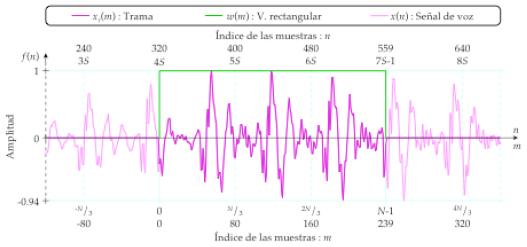
\includegraphics[width=0.75\textwidth]{Imagenes/Cap2/image035}
\end{center}
\begin{center}
\vskip -0.5cm
\caption{\small{Extracción de una trama mediante una ventana rectangular.}}
\label{fig:figura2.34}
{\small{Fuente: \cite{eyra}}}
\end{center}
\end{figure}

Sin embargo, la presencia de ésta ventana ocasiona la distorsión del espectro de la señal de voz, pero si se pondera la trama por una ventana con la forma adecuada, entonces se puede reducir la distorsión en la frecuencia, aunque se deforme la señal en el tiempo. En el reconocimiento de voz, la ventana que más se utiliza es la de Hamming:
\begin{equation}
\label{eq:ecuacion36}
%
w(n) = 
\begin{cases}
0 & \text{para $n < 0$} \\ 
0.54 - 0.46cos(\frac{2\pi n}{N-1}) & \text{para $0 \leq  n \leq  N-1$} \\ 
0 & \text{para $n > N-1$} 
\end{cases}
%
\end{equation}
La Figura \ref{fig:figura2.35} es la representación gráfica de la ventana de Hamming, la cual tiene valores que decaen suavemente hacia cero, aunque en los extremos, tiene una transición abrupta para el primer y el último valor de la ventana, los que son iguales a 0.08.

\begin{figure}[ht]
\begin{center}
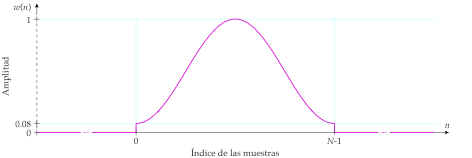
\includegraphics[width=0.6\textwidth]{Imagenes/Cap2/image036}
\end{center}
\begin{center}
\vskip -0.5cm
\caption{\small{Ventana de Hamming.}}
\label{fig:figura2.35}
{\small{Fuente: \cite{eyra}}}
\end{center}
\end{figure}
El segmento o la trama ponderada $x_{w}(n)$ se obtiene mediante el producto de cada una de las muestras de la trama de análisis $x_{l}(n)$ por el peso correspondiente de la ventana de Hamming $w(n)$:
\begin{equation}
\label{eq:ecuacion37}
\begin{aligned}
& x_{w}(n) = x_{l}(n) \cdot w(n) \\
& x_{w}(n) = x_{l}(n) \cdot \left [ 0.54 - 0.46cos\left ( \frac{2 \pi n}{N-1} \right ) \right ]
\end{aligned}
\qquad
n = 0,1,2,3,...,N-1
\end{equation}
\vskip 0.5cm
El ponderado de la trama de análisis contribuye a minimizar las discontinuidades al inicio y al final de las tramas, al atenuar los valores en los extremos. De otro modo la disparidad entre la primera y la última muestra de la trama ocasionaría algunos efectos indeseables en los valores del espectro en frecuencia. No obstante, si las muestras que se encuentran cerca de los extremos de la trama describen algún evento significativo de corta duración, entonces este evento prácticamente no afecta a la trama, dado que recibe un ponderado bajo. Así que normalmente, las tramas se traslapan para asegurar que todos estos eventos se tomen en cuenta al ser cubiertos en las tramas adyacentes.
\vskip 0.5cm
Otro aspecto importante es la selección de la longitud de la trama $N$, pues por lo general, el trabajo de computo requerido durante el análisis es proporcional a esta, por lo que resulta ventajoso mantenerla tan pequeña como sea posible. Sin embargo, se deben abarcar varios periodos del tono fundamental (pitch) para asegurar que los resultados sean confiables. Además, debido al ponderado, la longitud de la trama debe ser lo suficientemente larga como para que los efectos de atenuación de la ventana de Hamming no afecten seriamente los resultados. 
\vskip 0.5cm
Adicionalmente, la longitud o la duración de la trama se determina mediante un compromiso entre las resoluciones en el tiempo y en la frecuencia, ya que la longitud de la trama es proporcional a la resolución en frecuencia, pero inversamente proporcional a la resolución en el tiempo. De manera similar, el traslape es proporcional al número de tramas en la señal de voz, pero también es proporcional a la correlación de las tramas subsecuentes. Por lo tanto, se debe buscar un balance o compromiso entre estas características contrapuestas.
\vskip 0.5cm
Una manera para determinar $V$ (longitud de la trama N), es haciendo el producto de la duración de la trama $T$ por la frecuencia de muestreo $f_{s}$ de la señal de voz:
\begin{equation}
\label{eq:ecuacion38}
V = (T:f_{s})_{int}
\end{equation}
No obstante, como el número de muestras por trama $N$ debe ser un valor entero, se debe redondear o truncar el resultado. El número de muestras de separación entre tramas adyacentes $S$, generalmente se selecciona de tal manera que se obtenga una tasa de 100 tramas por segundo ($Fps = 100$), es decir una trama cada 10 ms.
\begin{equation}
\label{eq:ecuacion39}
Fps = \frac{f_{s}}{S} \hspace{1cm} \Rightarrow \hspace{1cm} S = \frac{f_{s}}{100}
\end{equation}
Los valores típicos de $V$ son de 10 a 30 ms. Las ventanas cortas han sido propuestas para estimar los parámetros del tracto vocal que varían rápidamente, mientras que las ventanas largas se usan para estimar la frecuencia del tono fundamental (pitch). Las tramas de 20 a 30 ms de duración generalmente tienen una buena relación entre ambas resoluciones, \cite{eyra}.
\vskip 0.5cm
Hasta aquí hemos visto todos los componentes que conforman el módulo de preprocesamiento, a continuación, veremos el módulo de entrenamiento.
\end{enumerate}

\subsubsection{Entrenamiento}
Para el entrenamiento se deben capturar diversas palabras recortadas por medio del módulo de preprocesamiento, mismas que representan las diferentes repeticiones. A partir de estas repeticiones se obtiene un conjunto de centroides que son almacenados en memoria. Para poder obtener estos centroides los valores numéricos obtenidos del preprocesamiento deben pasar por un algoritmo de extracción de características.
\begin{enumerate}
\item[a)]Extracción de características
\par
Es el proceso mediante el cual, dado un conjunto de datos se desea obtener otro conjunto de datos resumidos, pero que contengan solo la información necesaria de los datos de entrada. Una buena técnica de extracción de características garantiza que dichos datos obtenidos son únicos para una determinada entrada, es decir que para dos señales de entrada diferentes, se obtiene dos conjuntos de características diferentes, \cite{claudio}.
\vskip 0.5cm
Sin embargo, obtener características plenamente diferentes involucra que todas las señales sean diferentes, así se traten de dos palabras iguales, pero con diversas tonalidades y velocidades. Por lo tanto, la obtención de características debe de asegurarme, que en ambas señales existen características que son propias para ambas. De esta manera podemos obtener un grado de similaridad adecuado para el reconocimiento de la señal de voz.
\vskip 0.5cm
Entre muchas técnicas de extracción de características, podemos mencionar las siguientes:
\begin{enumerate}
\item[-]Algoritmo de características Fonético Acústicas
\item[-]Algoritmo basado en la Transformada de Fourier
\item[-]Codificación Predictiva Lineal (LPC)
\item[-]Coeficientes Cepstrales en Escala Mel (MFCC)
\item[-]Predicción Perceptual Lineal (PLP)
\item[-]Algoritmo basado en Wavelet.
\end{enumerate}

En \citep{unam}, se hace un análisis comparativo entre los algoritmos LPC, MFCC y PLP teniendo como resultado al MFCC como mejor algoritmo de extracción de características, ver la Figura \ref{fig:figura2.36}. En \citep{orlando}, se realiza una evaluación y comparación entre los Wavelets y los MFCC, resultando también a los MFCC con mejor desempeño, pero si bien tienen la misma complejidad computacional el tiempo de ejecución de los Wavelets es menor.

\newpage
\begin{figure}[ht]
\begin{center}
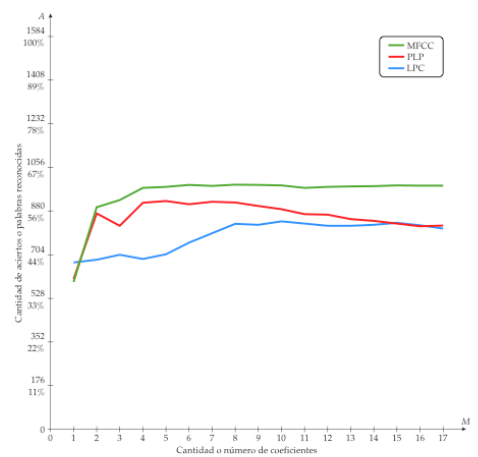
\includegraphics[width=0.55\textwidth]{Imagenes/Cap2/image037}
\end{center}
\begin{center}
\vskip -0.5cm
\caption{\small{Comparación de la variación en el reconocimiento entre LPC, MFCC Y PLP.}}
\label{fig:figura2.36}
{\small{Fuente: \cite{unam}}}
\end{center}
\end{figure}

Para este trabajo de Tesis teniendo lo anterior como antecedentes, hemos optado por la técnica MFCC (Coeficientes Cepstrales en la Frecuencia de Mel). La Figura \ref{fig:figura2.37} muestra el proceso del MFCC y como al final se retornan los cepstrum.

\begin{figure}[ht]
\begin{center}
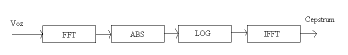
\includegraphics[width=0.5\textwidth]{Imagenes/Cap2/image038}
\end{center}
\begin{center}
\vskip -0.5cm
\caption{\small{Proceso de extracción de características con MFCC.}}
\label{fig:figura2.37}
{\small{Fuente: \cite{rabiner}}}
\end{center}
\end{figure}

\newpage
\item[b)]Codificación o análisis Mel cepstral
\par
En 1980 Davis y Mermelstein propusieron un nuevo tipo de representación del cepstrum, en el cual combinaron sus ventajas con los conocimientos de la percepción no lineal de la frecuencia en el sistema auditivo humano, tomando como base los estudios realizados por Zwicker en 1961. En este método de análisis, se utiliza la parte real del cepstrum, pero con una transformación no lineal de la frecuencia, pasando de la escala en Hertz a la escala de frecuencia Mel. Por eso, a estos coeficientes se les ha denominado como los Coeficientes Cepstral en la Frecuencia Mel o MFCC, \cite{eyra}.
\vskip 0.5cm
La mayor parte de los sistemas han estado convergiendo hacia el uso de estos vectores, que se obtienen a partir de un procesamiento de la señal de voz empleando un banco de filtros que ha sido diseñado tomando en cuenta algunas propiedades de la percepción del sonido en el sistema auditivo humano, con lo que se busca imitar su comportamiento.
\vskip 0.5cm
A continuación, se describe un procedimiento para obtener los coeficientes MFCC. La Figura \ref{fig:figura2.38} muestra el diagrama de bloques para este procedimiento. Los bloques muestran las operaciones necesarias y a la izquierda de éstos se muestran los parámetros de entrada requeridos en cada paso. A partir del cuarto bloque (ponderado por la ventana de Hamming), las operaciones se realizan sobre las tramas de la señal de voz. La consiguiente reducción en el número de parámetros para cada trama se ilustra mediante la cantidad de flechas.

\newpage
\begin{figure}[ht]
\begin{center}
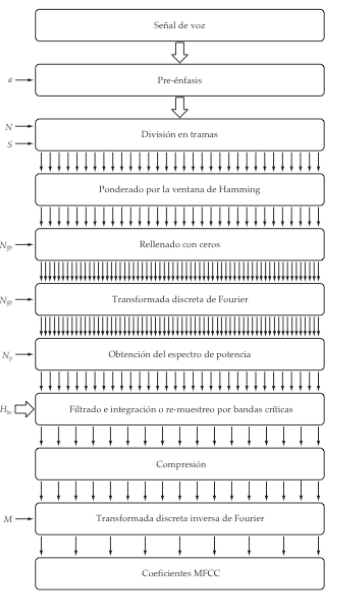
\includegraphics[width=0.4\textwidth]{Imagenes/Cap2/image039}
\end{center}
\begin{center}
\vskip -0.5cm
\caption{\small{Procedimiento para la obtención de los coeficientes MFCC.}}
\label{fig:figura2.38}
{\small{Fuente: \cite{eyra}}}
\end{center}
\end{figure}

Las etapas preénfasis, división de tramas y ponderado por la ventana de Hamming ya las vimos en la etapa de preprocesamiento, por lo que solamente veremos las etapas restantes.

\newpage
\begin{enumerate}
\item[•]Transformada discreta de Fourier
\par
El espectro en frecuencia de una señal discreta se puede estimar mediante DFT (Transformada Discreta de Fourier):
\begin{equation}
\label{eq:ecuacion40}
X(k) = \sum_{n=0}^{N-1}x(n)e^{-j\frac{2\pi nk}{N}}
\end{equation}
Esta transformada proporciona un conjunto de $N$ valores en el dominio de la frecuencia, en donde $X(k)$ es la transformada discreta de Fourier en el dominio de la frecuencia, de la señal discreta $x(n)$ en el dominio del tiempo. Sin embargo, en la práctica, la transformada discreta de Fourier se calcula de una manera mucho más eficiente mediante FFT (Transformada Rápida de Fourier).

\item[•]Rellenado con ceros
\par
Para facilitar el uso de la transformada rápida de Fourier, la longitud de la trama $N$ debería de ser igual al número de puntos para la transformada rápida de Fourier $N_{fft}$, un número que debe ser igual a la potencia de dos más próxima:
\begin{equation}
\label{eq:ecuacion41}
N_{fft} = 2^{[log_{2}(N)]_{int}}
\end{equation}
Pero si no se cumple con esta condición, entonces se puede rellenar con ceros, es decir, añadir las muestras nulas que hagan falta.
\vskip 0.5cm
\begin{equation}
\label{eq:ecuacion42}
x_{zp}(n)= \left\{ \begin{array}{lcl}
x_{w}(n) & \mbox{ para } & n = 0,1,2,3,...,N-1 \\
& & \\
0 & \mbox{ para } & n = N,N+1,...,N_{fft} - 1
\end{array}
\right.
\end{equation}
\vskip 0.5cm
A partir de la Ecuación \eqref{eq:ecuacion40} de la transformada discreta de Fourier se tiene:
\begin{equation}
\label{eq:ecuacion43}
X(k) = \sum_{n=0}^{N_{fft}-1}x(n)e^{-j\frac{2\pi nk}{N_{fft}}}
\end{equation}
Se puede apreciar que el agregar valores nulos a $x(n)$ no afecta significativamente la sumatoria para cualquier $X(k)$. Sin embargo, la longitud aumentada de la trama $N_{fft}$ solamente proporciona una mejor descripción de la transformada discreta de Fourier, pues no incrementa la resolución en frecuencia, pues este es el único propósito de la longitud de la trama $N$.

\item[•]Obtención del espectro de frecuencia
\par
El espectro en frecuencia de una trama de análisis se obtiene mediante el algoritmo FFT (Transformada Rápida de Fourier):
\begin{equation}
\label{eq:ecuacion44}
X(k) = \mathbf{FFT}\{ x_{zp}(n), N_{fft} \}
\qquad
\begin{aligned}
& k = 0,1,2,3,...,N_{fft}-1 \\
& n = 0,1,2,3,...,N_{fft}-1
\end{aligned}
\end{equation}
Dado que la señal de voz $x(n)$ es una secuencia de números reales, $X(k)$ y $X(N - k)$ son conjugados complejos. Puesto que la magnitud de los conjugados complejos es igual, el espectro en frecuencia resultante tiene una simetría par con respecto a la mitad de la frecuencia de muestreo, es decir, que la magnitud de la mitad superior del espectro es un reflejo de la mitad inferior.

\item[•]Obtención del espectro de potencia
\par
Ahora bien, no importa tanto la respuesta en frecuencia, sino la envolvente de la respuesta en frecuencia. Las características del tracto vocal se pueden estimar mediante el espectro de potencia $P(k)$ que se calcula como la magnitud del espectro al cuadrado o la suma de los cuadrados de la parte real e imaginaria del espectro:
\begin{equation}
\label{eq:ecuacion45}
\begin{aligned}
& P(k) = \left | X(k) \right |^{2} \\
& P(k) = \mathbf{real}[X(k)]^{2} + \mathbf{imag}[X(k)]^{2}
\end{aligned}
\qquad
k = 0,1,2,3,...,N_{fft}-1
\end{equation}
El espectro de potencia se compone de valores reales, enfatiza los picos en el espectro y conserva la simetría par del espectro en frecuencia. Por lo tanto, normalmente solamente se ocupa la mitad inferior del espectro, es decir los primeros $N_{p}$ valores:
\begin{equation}
\label{eq:ecuacion46}
\begin{aligned}
& N_{p} = 0.5N_{fft} \\
& P(k) = \mathbf{real}[X(k)]^{2} + \mathbf{imag}[X(k)]^{2} \qquad k = 0,1,2,3,...,N_{p}
\end{aligned}
\end{equation}
Hay que destacar que el espectro de potencia solamente proporciona información acerca de la magnitud, pues la información relacionada con la fase se descarta. Esto es consistente con el hecho de que la fase no aporta ninguna información que resulte útil. De hecho, se ha comprobado experimentalmente que la percepción de una señal reconstruida con una fase distinta es prácticamente indistinguible de la señal original, esto si se mantiene la continuidad secuencial de la fase entre las tramas.

\item[•]Cambio de la escala de frecuencia
\par
Existen muchas formas diferentes para las ventanas que se pueden emplear en los bancos de filtros, pero todas estas se basan en alguna escala de frecuencia que se considera aproximadamente lineal para frecuencias menores de 1000 Hz, pero para frecuencias mayores que ésta, presenta un comportamiento no lineal (logarítmico).
\vskip 0.5cm
Este cambio en la escala de frecuencia en inglés se denomina \textit{frequency warping}, es decir, que se realiza un arqueado o una transformación de la escala de frecuencia en Hertz, a otra escala de frecuencia que exhibe un comportamiento logarítmico. Las escalas Mel, que es la que usaremos en esta tesis, y Bark son dos ejemplos, puesto que están basadas en datos experimentales de la percepción humana, existen varias aproximaciones que se pueden usar para estas.
\vskip 0.5cm
La escala Mel fue propuesta por Stevens, Volksman y Newmann en 1940. Un Mel es una unidad de medición de la frecuencia o del tono percibido, esta no corresponde de manera lineal a la frecuencia real del tono. Se designó como punto inicial de referencia, que una frecuencia de 1000 Hz también es de 1000 Mels. 
\vskip 0.5cm
Los observadores juzgan tonos espaciados exponencialmente como tonos equiespaciados. De esta manera fue posible determinar un mapeo entre la escala de la frecuencia real (Hertz) y la escala de la frecuencia percibida (Mels).
\vskip 0.5cm
La siguiente ecuación proporciona una equivalencia entre la escala logarítmica de la frecuencia Mel $f_{mel}$ con respecto a la escala de frecuencia en Hertz $f_{Hz}$:
\begin{equation}
\label{eq:ecuacion47}
f_{mel}(f_{Hz}) = \frac{1000}{\mathbf{Ln}(2)}\mathbf{Ln}\left ( 1 + \frac{f_{Hz}}{1000} \right )
\end{equation}
No obstante, se acostumbra utilizar otra función de aproximación para realizar la transformación no lineal de la frecuencia en Hertz a la escala de frecuencia Mel:
\begin{equation}
\label{eq:ecuacion48}
f_{mel}(f_{Hz}) = 1125\mathbf{Ln}\left ( 1 + \frac{f_{Hz}}{700} \right )
\end{equation}
La Figura \ref{fig:figura2.40} muestra la representación gráfica de la ecuación anterior, en donde se puede apreciar el arqueado de la frecuencia al cambiar de la escala lineal de frecuencia en Hertz $f_{Hz}$ a la escala logarítmica de la frecuencia Mel $f_{mel}$:
\begin{figure}[H]
\begin{center}
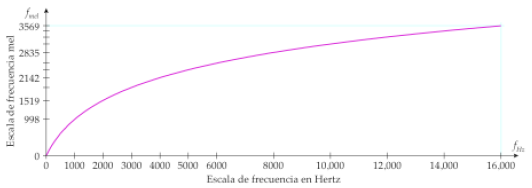
\includegraphics[width=0.65\textwidth]{Imagenes/Cap2/image041}
\end{center}
\begin{center}
\vskip -0.5cm
\caption{\small{Gráfica del arqueado de la frecuencia con la escala Mel.}}
\label{fig:figura2.40}
{\small{Fuente: \cite{eyra}}}
\end{center}
\end{figure}

\newpage
\item[•]Definición de las bandas criticas triangulares con la escala Mel
\par
El diseño de los filtros para las bandas críticas primero se realiza en la escala Mel. Los filtros utilizados en este método presentan una forma triangular, que es simétrica con respecto a su frecuencia central y tienen el mismo ancho de banda en la escala Mel.
\vskip 0.5cm
Aunque a estas ventanas triangulares se les suele llamar filtros, estas simplemente se usan para promediar el espectro de potencia con respecto a la frecuencia central de cada una de las bandas críticas. La función que las define está dada por la siguiente ecuación y su representación gráfica se muestra en la Figura \ref{fig:figura2.41}.
\begin{equation}
\label{eq:ecuacion49}
H_{bc}(f)= \left\{ \begin{array}{lcl}
0 & \mbox{ para } & f \leq f_{l} \\
& & \\
\frac{1}{(f_{c} - f_{l})}(f - f_{l}) & \mbox{ para } & f_{l} < f < f_{c} \\
& & \\
1 & \mbox{ para } & f = f_{c} \\
& & \\
\frac{- 1}{(f_{h} - f_{c})}(f - f_{h}) & \mbox{ para } & f_{c} < f < f_{h} \\
& & \\
0 & \mbox{ para } & f \geq f_{h} \\
\end{array}
\right.
\end{equation}

\begin{figure}[H]
\begin{center}
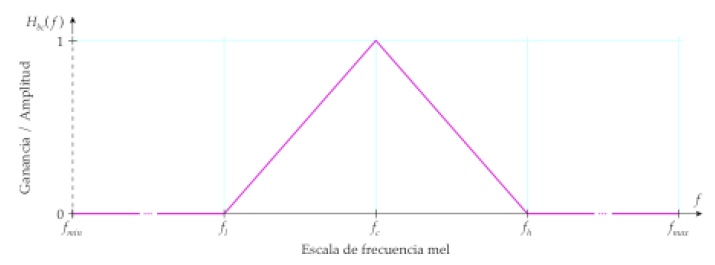
\includegraphics[width=0.5\textwidth]{Imagenes/Cap2/image042}
\end{center}
\begin{center}
\vskip -0.5cm
\caption{\small{Curva para las bandas críticas triangulares.}}
\label{fig:figura2.41}
{\small{Fuente: \cite{eyra}}}
\end{center}
\end{figure}

En la Ecuación \eqref{eq:ecuacion49} se puede apreciar que los primeros términos (cocientes) son las pendientes de las rectas que forman la ventana triangular, y los otros términos del producto contienen a la variable independiente con su respectiva abscisa al origen. Ahora bien, la transformación no lineal de la frecuencia en Hertz a la escala de frecuencia Mel, se acostumbra realizar mediante la función de aproximación Ecuación \eqref{eq:ecuacion48}.
\vskip 0.5cm
El rango de frecuencias de interés abarca desde los 0 Hz hasta la frecuencia de Nyquist, sin embargo, se puede determinar un límite inferior de frecuencia $f_{min}$, y un límite superior de frecuencia $f_{max}$. Para la señal de voz, se recomienda que $f_{min} > 100 Hz$ y que el límite superior de frecuencia sea menor a la frecuencia de Nyquist, aunque para una frecuencia mayor de 6800 Hz ya no hay mucha información en la señal de voz. Además, si se fija el límite inferior de frecuencia arriba de 50 o 60 Hz, se puede evitar el ruido procedente de la red de suministro o distribución de AC. Ahora bien, puesto que estos límites están definidos en Hertz, hace falta transformarlos a la escala Mel.
\begin{equation}
\label{eq:ecuacion50}
\left ( f_{min} \right )_{mel} = 1125\mathbf{Ln}\left ( 1 + \frac{f_{min}}{700} \right )
\qquad
\left ( f_{max} \right )_{mel} = 1125\mathbf{Ln}\left ( 1 + \frac{f_{max}}{700} \right )
\end{equation}
Las frecuencias centrales deben estar equiespaciadas en la escala Mel, entonces se puede calcular la separación en frecuencia entre éstas $SF$, mediante la siguiente fórmula:
\begin{equation}
\label{eq:ecuacion51}
SF = \frac{\left ( f_{max} \right )_{mel} - \left ( f_{min} \right )_{mel}}{BC + 1}
\end{equation}
\newpage
Las frecuencias centrales están separadas por múltiplos enteros de este parámetro más el valor del límite inferior de frecuencia:
\begin{equation}
\label{eq:ecuacion52}
f_{c}(bc)_{mel} = bc \cdot SF + \left ( f_{min} \right )_{mel}
\qquad
bc = 1,2,3,...,BC
\end{equation}
En donde $bc$ denota el número correspondiente de la banda crítica. Ahora sólo hace falta transformar las frecuencias centrales de la escala Mel a la escala en Hertz mediante la siguiente fórmula, que es la función inversa de la Ecuación \eqref{eq:ecuacion48}
\begin{equation}
\label{eq:ecuacion53}
f_{Hz}(f_{mel}) = 700\left [ e^{\left ( \frac{f_{mel}}{1125} \right )} - 1 \right]
\end{equation}
Con estos valores de las frecuencias centrales en Hertz, ya se pueden determinar las frecuencias inferior y superior para cada una de las bandas críticas. La frecuencia inferior para una banda crítica $bc$ es igual a la frecuencia central de la banda crítica anterior:
\begin{equation}
\label{eq:ecuacion54}
f_{l}(bc) = f_{c}(bc - 1)
\end{equation}
La frecuencia superior para una banda crítica es igual a la frecuencia central de la banda crtica posterior:
\begin{equation}
\label{eq:ecuacion55}
f_{h}(bc) = f_{c}(bc + 1)
\end{equation}
La frecuencia inferior de la primera banda crítica es igual al límite inferior de frecuencia Ecuación \ref{eq:ecuacion56}, de manera similar, la frecuencia superior de la última banda crítica es igual al límite superior de frecuencia Ecuación \ref{eq:ecuacion57}.
\begin{equation}
\label{eq:ecuacion56}
f_{l}(1) = f_{min}
\end{equation}

\begin{equation}
\label{eq:ecuacion57}
f_{h}(BC) = f_{max}
\end{equation}

En la Figura \ref{fig:figura2.42} se muestra la representación gráfica, en la escala Mel con banco de filtros $BC = 17$, limite inferior de frecuencia $f_{min} = 0 Hz$ y limite superior de frecuencia $f_{max} = 4000 Hz$, podemos ver que las bandas críticas están equiespaciadas y todas las bandas críticas tienen el mismo ancho de banda.
\begin{figure}[H]
\begin{center}
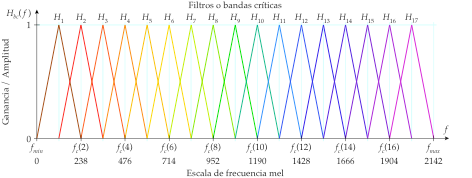
\includegraphics[width=0.53\textwidth]{Imagenes/Cap2/image043}
\end{center}
\begin{center}
\vskip -0.5cm
\caption{\small{Banco de filtros o ventanas triangulares equiespaciados en la escala Mel.}}
\label{fig:figura2.42}
{\small{Fuente: \cite{eyra}}}
\end{center}
\end{figure}
\vskip -0.5cm
La Figura \ref{fig:figura2.43} muestra el mismo banco de filtros, pero ahora en la escala en Hertz. Puede apreciarse como la distribución de las bandas críticas ahora sigue una distribución logarítmica y también como se incrementa el ancho de banda al aumentar la frecuencia.
\begin{figure}[H]
\begin{center}
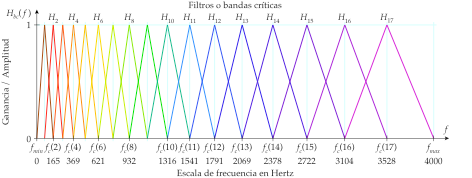
\includegraphics[width=0.53\textwidth]{Imagenes/Cap2/image044}
\end{center}
\begin{center}
\vskip -0.5cm
\caption{\small{Banco de filtros o ventanas triangulares en Hertz con distribución logarítmica.}}
\label{fig:figura2.43}
{\small{Fuente: \cite{eyra}}}
\end{center}
\end{figure}
\newpage
Finalmente, falta hacer un muestreo de las bandas críticas de acuerdo al número de puntos del espectro de potencia $N_{p}.$ Ahora bien, como las bandas críticas contienen unos cuantos valores diferentes de cero, no hace falta calcular todos los valores correspondientes a cada uno de los puntos del espectro de potencia, basta con las muestras comprendidas entre la frecuencia inferior y la superior para cada banda crítica.
\vskip 0.5cm
A cada muestra del espectro de potencia $P(k)$ le corresponde un valor de frecuencia en Hertz, el cual es un múltiplo de la resolución en frecuencia del espectro:
\begin{equation}
\label{eq:ecuacion58}
f = k \cdot \Delta f
\qquad
k = 0,1,2,3,...,N_{p}
\end{equation}
La resolución en frecuencia del espectro $\Delta f$, se puede calcular mediante el cociente de la frecuencia de muestreo $f_{s}$, entre el número de puntos para la transformada rápida de Fourier $N_{fft}$:
\begin{equation}
\label{eq:ecuacion59}
\Delta f = \frac{f_{s}}{N_{fft}}
\end{equation}
Si se invierte este cociente, el nuevo factor es la resolución por muestra del espectro:
\begin{equation}
\label{eq:ecuacion60}
\Delta k = \frac{N_{fft}}{f_{s}}
\end{equation}
El cual se puede utilizar para determinar que índice o muestra corresponde a determinada frecuencia, al multiplicar esa frecuencia por este factor de equivalencia:
\begin{equation}
\label{eq:ecuacion61}
k = \left ( f \cdot \Delta k  \right )_{\mathbf{int}}
\end{equation}
Puesto que los índices de las muestras deben ser números enteros, se tiene que redondear el resultado a un número entero. El índice para la frecuencia inferior $k_{l}$ se puede redondear hacia arriba, pero el índice para la frecuencia superior $k_{h}$ se puede redondear hacia abajo. También, si es necesario, hay que tomar en cuenta que la primera muestra del espectro de potencia representa a la frecuencia cero.
\vskip 0.5cm
Con los índices correspondientes a las frecuencias inferior $k_{l}$ y superior $k_{h}$, ya se pueden calcular los $N_{bc}$ valores diferentes de cero para cada una de las bandas críticas.
\begin{equation}
\label{eq:ecuacion62}
N_{bc} = k_{h}(bc) - k_{l}(bc) + 1
\end{equation}
Para esto, primero se obtiene el valor correspondiente en frecuencia para la muestra $k$, comprendida dentro del intervalo $k_{l}(bc) \leq k \leq k_{h}(bc)$ de una banda crítica $bc$. Entonces, el valor correspondiente a la muestra $k$ para el filtro o la banda crítica $H_{bc}$ se determina mediante la Ecuación \eqref{eq:ecuacion58}, según sea el caso.

\item[•]Compresión
\par
En lugar de simplemente usar la magnitud del espectro remuestreado mediante la escala Mel para calcular los MFCC, algunos investigadores han sugerido que es más provechoso el emplear una función logaritmo para calcular la energía total de las bandas críticas alrededor de las frecuencias centrales:
\begin{equation}
\label{eq:ecuacion63}
P_{sc}(bc) = \mathbf{log}[P_{s}(bc)]
\qquad
bc = 1,2,3,...,BC
\end{equation}
El procesamiento de la magnitud y la obtención de su logaritmo también se realizan en el oído humano. Es más, el empleo de la magnitud descarta la información innecesaria que proporciona la fase mientras que el logaritmo efectúa una compresión, dando como resultado que la extracción de características sea menos sensible a las variaciones de la amplitud producidas por las resonancias espectrales.

\item[•]Transformada inversa de Fourier
\par
El último paso en el cálculo de los MFCC consiste en realizar la transformada discreta inversa de Fourier del espectro muestreado y comprimido $P_{sc}$. En este paso es donde se obtienen los MFCC, además esta etapa del procedimiento tiene grandes ventajas, puesto que los valores del espectro son números reales y presentan una simetría par con respecto a la frecuencia de Nyquist, entonces se puede reducir a una DCT (Transformada Coseno Discreta) en lugar de la IFFT (Transformada Discreta Inversa de Fourier):
\begin{equation}
\label{eq:ecuacion64}
c_{m} = \sum_{bc = 1}^{BC}P_{sc}(bc)\mathbf{cos}\left [ \frac{\pi }{BC}\left ( bc - \frac{1}{2} \right ) m \right ]
\qquad
m = 0,1,2,3,...,M
\end{equation}
La transformada coseno discreta tiene la propiedad de producir características que prácticamente no están correlacionadas entre sí. De tal manera que se pueden usar matrices diagonales de covarianza en lugar de las matrices ordinarias de covarianza, con lo que se reduce en gran manera el trabajo de cómputo y el número de parámetros a estimar. Además, la transformada coseno discreta proporciona un suavizado del espectro si solamente se conservan los primeros coeficientes.
\vskip 0.5cm
Por lo tanto, la solución final es el vector o el conjunto de coeficientes MFCC:
\begin{equation}
\label{eq:ecuacion65}
\begin{aligned}
& \mathbf{V}_{mfcc} = C_{m} \\
& \mathbf{V}_{mfcc} = [C_{1},C_{2},C_{3},...,C_{M}]
\end{aligned}
\qquad
m = 1,2,3,...,M
\end{equation}
El coeficiente inicial $c_{0}$ representa el logaritmo de la energía promedio en la trama y se descarta, pues ésta se puede calcular directamente a partir de la señal de voz.

\item[•]Coeficientes delta y doble deltas
\par
Los cambios temporales en el espectro, tienen una importancia significativa en la percepción humana, una manera de capturar estos cambios es utilizando los coeficientes delta cuya finalidad es medir el cambio de los coeficientes en el tiempo, \cite{xuedong}. Las características a usar en un reconocedor usando MFCC con $F_{s}$ de 16 KHz, es la siguiente:
\vskip 0.5cm
Por frame analizado (ventaneamiento) se tendrá un vector $X_{k}$ , donde:
\begin{equation}
\label{eq:ecuacion66}
X_{k} = 
\begin{pmatrix}
C_{k}\\ 
\Delta C_{k}\\ 
\Delta \Delta C_{k}
\end{pmatrix}
\end{equation}

\begin{enumerate}
\item[-]$C_k$ son los 13 coeficientes MFCC 
\item[-]13 coeficientes delta MFCC
\begin{equation}
\label{eq:ecuacion67}
\Delta C_{k} = C_{k + 2} - C_{k - 2}
\end{equation}
\item[-]13 coeficientes doble delta MFCC
\begin{equation}
\label{eq:ecuacion68}
\Delta \Delta C_{k} = \Delta C_{k + 1} - \Delta C_{k - 1}
\end{equation}
\end{enumerate}
\end{enumerate}
\end{enumerate}

\subsubsection{Reconocimiento}
Una vez terminada la fase de extracción de características, debemos empezar con la tarea del reconocimiento automático. Al igual que en la extracción de características, el proceso de reconocer una señal de voz por una persona también es motivo del estudio de múltiples algoritmos que realizan esta tarea, tales como el DTW (Alineamiento Temporal Dinámico), HMM (Modelos Ocultos de Markov), ANN (Redes Neuronales), etc. ver en \citep{luna}. 
\vskip 0.5cm
Este bloque dentro de los sistemas de reconocimiento de locutor, consiste en la comparación de parámetros característicos o patrones de voz. Como se explicó en el diagrama de bloques en la Figura \ref{fig:figura2.6}, es necesario hacer la comparación de patrones de referencia contra los patrones de prueba y en base a una lógica de decisión reconocer al locutor.
\vskip 0.5cm
Una característica fundamental de los sistemas de reconocimiento es la forma en que los vectores característicos son combinados y comparados con los patrones de referencia. Para poder realizar estas operaciones es necesario definir una medida de distancia o distorsión entre los vectores característicos. Si las características a medir tienen la misma longitud, pues es fácil realizar esta operación. Sin embargo, el problema se presenta si tenemos dos patrones que corresponden a la misma palabra, pero pronunciadas a diferentes velocidades, este análisis se hace inadecuado. Es por ello que para esta tesis emplearemos la técnica de \textit{Alineamiento Temporal Dinámico} (DTW) para comparar estos patrones, la cual a su vez servirá para construir los patrones de referencia.
\newpage
\begin{enumerate}
\item[a)]Alineamiento Temporal Dinámico
\par
Si se consideran dos patrones de voz, $X$ y $Y$, representados por las secuencias ($x_{1}, x_{2},..., x_{n}$) y ($y_{1}, y_{2},..., y_{m}$) respectivamente, donde $x_{n}$ y $y_{m}$ son vectores que contienen los parámetros característicos de cada segmento de voz analizado, $N$ y $M$ son el número de segmentos en cada palabra y no necesariamente $N = M$. 
\vskip 0.3cm
El propósito del alineamiento en el tiempo de patrones de voz es el de obtener una función de alineamiento $w$ entre los índices temporales $n$ y $m$ con la cual se logre una correspondencia entre los patrones de voz de la palabra de prueba y los patrones de voz de la palabra de referencia. En la Figura \ref{fig:figura2.45}, se muestra un ejemplo de lo anterior donde se tienen los patrones de voz de la palabra de referencia en el eje de las ordenadas y los patrones de voz de la palabra de prueba en el eje de las abscisas. Se observa cómo la función de alineamiento proporciona una correspondencia entre los vectores $x_{n}$ y $y_{m}$ de los patrones de voz.
\begin{figure}[H]
\begin{center}
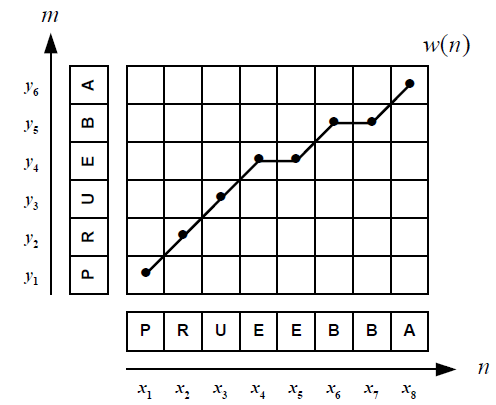
\includegraphics[width=0.35\textwidth]{Imagenes/Cap2/image046}
\end{center}
\begin{center}
\vskip -0.5cm
\caption{\small{Ejemplo de alineación de patrones de voz.}}
\label{fig:figura2.45}
{\small{Fuente: \cite{rabiner}}}
\end{center}
\end{figure}

\newpage
\begin{equation}
\label{eq:ecuacion70}
M_{1} = w(N_{1})
\end{equation}
\begin{equation}
\label{eq:ecuacion71}
M_{2} = w(N_{2})
\end{equation}
La función de alineamiento debe cumplir con las Ecuaciones \eqref{eq:ecuacion70} y \eqref{eq:ecuacion71}, a estas condiciones se les llama conjunto restringido en los límites, además de cumplir con ciertas suposiciones acerca de la forma de $w(n)$. Por ejemplo, si $w(n)$ es una función lineal, el alineamiento en el tiempo es simplemente una compresión o expansión de una escala en el tiempo. Esta función lineal asume que la variación en la pronunciación de una palabra es proporcional a la duración de la misma y es independiente del sonido hablado y por consiguiente no modela adecuadamente la forma en que se pronuncia una palabra, sobre todo no modela las variaciones de velocidad con que se pronuncian los sonidos vocales, por lo que es necesario emplear una función de alineamiento no lineal entre los patrones de voz.
\vskip 0.5cm
Un enfoque más sofisticado y poderoso para alinear en el tiempo, consiste en restringir a $w(n)$ para que satisfaga un conjunto de condiciones locales de continuidad,
\begin{equation}
\label{eq:ecuacion72}
w(n+1) - w(n) = 0,1,2(w(n) \neq w(n-1))
\end{equation}
\begin{equation}
\label{eq:ecuacion73}
w(n+1) - w(n) = 1,2(w(n) = w(n-1))
\end{equation}
estas ecuaciones hacen que $w(n)$ sea monotónicamente creciente con una pendiente máxima de 2 y una pendiente mínima de 0, excepto cuando la pendiente anterior fue 0, en tal caso la pendiente mínima será de 1. 
\vskip 0.3cm
Las condiciones de las Ecuaciones \eqref{eq:ecuacion70} y \eqref{eq:ecuacion71} junto con las condiciones de continuidad de las Ecuaciones \eqref{eq:ecuacion72} y \eqref{eq:ecuacion73} limitan a la función de alineamiento a seguir una trayectoria dentro del paralelogramo formado en el plano $(n, m)$ como se muestra en la Figura \ref{fig:figura2.46}. Los vértices, $A$ y $B$, del paralelogramo se obtiene de la intersección de las líneas,
\begin{equation}
\label{eq:ecuacion74}
\begin{aligned}
& m - 1 = 2(n - 1) \\
& m - M = (n - N)/2
\end{aligned}
\qquad
\text{Vértice A}
\end{equation}
y
\begin{equation}
\label{eq:ecuacion75}
\begin{aligned}
& m - 1 = (n - 1)/2 \\
& m - M = 2(n - N)
\end{aligned}
\qquad
\text{Vértice B}
\end{equation}

La función de alineamiento $w(n)$, está restringida a seguir una trayectoria dentro de la región sombreada de la Figura \ref{fig:figura2.46}.
\begin{figure}[H]
\begin{center}
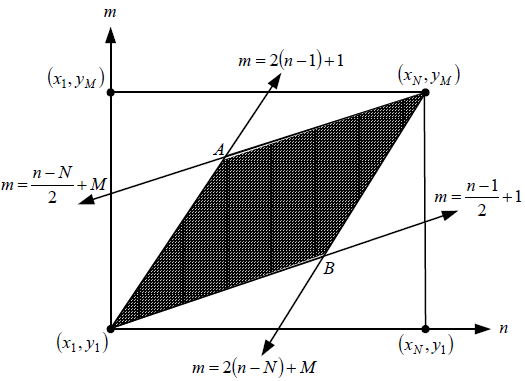
\includegraphics[width=0.43\textwidth]{Imagenes/Cap2/image047}
\end{center}
\begin{center}
\vskip -0.5cm
\caption{\small{Región de posibles trayectorias de la función de alineamiento.}}
\label{fig:figura2.46}
{\small{Fuente: \cite{rabiner}}}
\end{center}
\end{figure}
\newpage
Para obtener la trayectoria de la función de alineamiento es necesario considerar una medida de similitud o distancia entre $X$ y $Y$, la cual se define considerando una distancia local $d(x_{n},y_{m})$. Esta distancia local se calcula para todos los vectores en el eje $n$ contra todos los vectores en el eje $m$ como se muestra en la Figura \ref{fig:figura2.47}. Por simplicidad esta distancia local será denotada como $d(n, m)$, donde $n = 1,2,...,N$, $m = 1,2,...,M$ y generalmente $N \neq M$. Entre más pequeño sea el valor de $d$, mayor es la similitud entre $x_{n}$ y $y_{m}$.
\begin{figure}[H]
\begin{center}
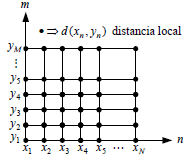
\includegraphics[width=0.3\textwidth]{Imagenes/Cap2/image048}
\end{center}
\begin{center}
\vskip -0.5cm
\caption{\small{Distancias locales generadas por los patrones de voz.}}
\label{fig:figura2.47}
{\small{Fuente: \cite{rabiner}}}
\end{center}
\end{figure}
\vskip -0.5cm
Dada la función de distancia local $d$, la trayectoria óptima de la función de alineamiento $w(n)$ acotada por el paralelogramo de la Figura \ref{fig:figura2.46}, debe de ser tal que la distancia acumulada total $D_{T}$ desde el punto $(x_{1}, y_{1})$ al punto $(x_{N}, y_{M})$ siguiendo a $w(n)$ sea mínima, es decir: 
\begin{equation}
\label{eq:ecuacion76}
D_{T} = \underset{\{w(n)\}}{min} \sum_{n=1}^{N}d(n,w(n))
\end{equation}
Donde $d(n,w(n))$ es la distancia local entre el segmento $n$ del patrón de referencia y el segmento $w(n)$ del patrón de prueba.
\vskip 0.5cm
Hasta este punto se ha mencionado la trayectoria óptima de la función de alineamiento, sin embargo, no se ha establecido un método para obtenerla. La técnica para determinarla es mediante el método de programación dinámica. Usando esta técnica, la distancia mínima acumulada a cualquier punto en el plano $(n,m)$ puede ser determinada en forma recursiva:
\begin{equation}
\label{eq:ecuacion77}
D_{A}(n,m) = d(n,m) + \underset{q \leq m}{min} D_{A}(n-1,q)
\qquad
\begin{aligned}
& n = 1,2,...,N \\
& m = 1,2,...,M
\end{aligned}
\end{equation}
\vskip 0.5cm
Donde $D_{A}(n-1, q)$ es la distancia mínima acumulada al punto $(n-1, q)$, y $q$ puede tomar valores de $q = m, m - 1, m - 2$. Dadas las restricciones de continuidad de las Ecuaciones \eqref{eq:ecuacion72} y \eqref{eq:ecuacion73} y la Ecuación \eqref{eq:ecuacion77} puede ser escrita de la siguiente forma:
\begin{equation}
\label{eq:ecuacion78}
\begin{aligned}
D_{A}(n,m) = d(n,m) + min[D_{A}(n-1,m)g(n-1,m) , \\
D_{A}(n-1,m-1),D_{A}(n-1,m-2)]
\end{aligned}
\end{equation}

Donde:
\vskip 0.2cm
\begin{center}
$
g(n,m) = \left\{ \begin{array}{lcl}
1 & w(n) \neq w(n-1) \\
& \\
\infty & w(n) = w(n-1) \\
\end{array}
\right.
$
\end{center}
\vskip 0.2cm
En la Figura \ref{fig:figura2.48}, se muestra un ejemplo gráfico de las restricciones de continuidad, además, se muestra una restricción no lineal ya que si la mejor trayectoria al punto $(n - 1, m)$ viene del punto $(n - 2, m)$, entonces ninguna trayectoria puede salir del punto $(n - 1, m)$, a estas restricciones se les conoce como restricciones locales del tipo Itakura.
\begin{figure}[H]
\begin{center}
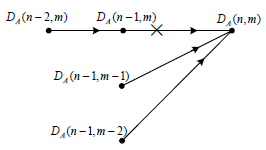
\includegraphics[width=0.35\textwidth]{Imagenes/Cap2/image049}
\end{center}
\begin{center}
\vskip -0.5cm
\caption{\small{Conjunto de posibles trayectorias hacia el punto (n, m).}}
\label{fig:figura2.48}
{\small{Fuente: \cite{rabiner}}}
\end{center}
\end{figure}
\vskip -1.0cm
La función de alineamiento se obtiene a partir de la Ecuación \eqref{eq:ecuacion77}. Esta función contiene los índices $m$ donde $D_{A}(n - 1, q)$ es mínima para $q = m, m-1, m-2$ y $n = 2,3,...,N$, en otras palabras, la función de alineamiento contiene los índices para los cuales existe una correspondencia entre el índice $n$ del patrón de referencia y el índice $m$ del patrón de prueba. La iteración de la ecuación se realiza para todos los índices $m$ válidos, es decir, todos los índices $m$ dentro del paralelogramo de la Figura \ref{fig:figura2.46}, y para cada valor de $n$, desde $n = 1$ hasta $n = N$. La solución final o distancia total está dada como:
\begin{equation}
\label{eq:ecuacion79}
D_{T} = D_{A}(N,M)
\end{equation}
Las Ecuaciones \eqref{eq:ecuacion78} y \eqref{eq:ecuacion79} definen la técnica de programación dinámica para el alineamiento en el tiempo de patrones de voz. Al aplicarla a dos patrones de voz, se obtiene la medida de distancia total y la función de alineamiento. La función de alineamiento se usa en la etapa de entrenamiento, mientras que la distancia total entre los patrones de voz se emplea en la etapa de prueba.
\vskip 0.5cm
A este método de alineación en el tiempo se le conoce como inicio y fin con restricción, rango de la pendiente 2 a 1 (Constrained Endpoints 2 to 1 slope range, CE2-1) donde se asume que existe un alineamiento perfecto entre los puntos de inicio y fin de los patrones de voz de prueba y referencia. En la Figura \ref{fig:figura2.49}, se ilustra este método.
\begin{figure}[H]
\begin{center}
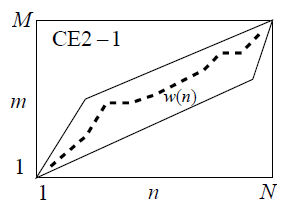
\includegraphics[width=0.3\textwidth]{Imagenes/Cap2/image050}
\end{center}
\begin{center}
\vskip -0.5cm
\caption{\small{Técnica de alineación dinámica en el tiempo CE2-1.}}
\label{fig:figura2.49}
{\small{Fuente: \cite{rabiner}}}
\end{center}
\end{figure}
\vskip -0.5cm
Existen dos variantes del método explicado anteriormente. La primera variante se le conoce como inicio y fin sin restricción, rango de la pendiente 2 a 1 (Unconstrained Endpoints 2 to 1 slope range, UE2-1), ver la Figura \ref{fig:figura2.50}, se utiliza cuando se tiene cierto grado de incertidumbre en la detección del inicio y fin de la palabra. 
\vskip 0.2cm
\begin{figure}[H]
\begin{center}
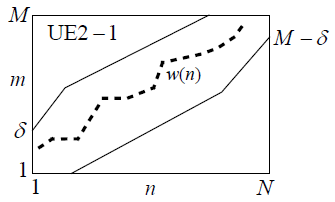
\includegraphics[width=0.35\textwidth]{Imagenes/Cap2/image051}
\end{center}
\begin{center}
\vskip -0.5cm
\caption{\small{Técnica de alineación dinámica en el tiempo UE2-1.}}
\label{fig:figura2.50}
{\small{Fuente: \cite{rabiner}}}
\end{center}
\end{figure}
\vskip -0.5cm
La segunda variante se le conoce como inicio y fin sin restricción, mínimos locales (Unconstrained Endpoints Local Mínimum, UELM), ver la Figura \ref{fig:figura2.51}. En este método, $w(n)$ se restringe a seguir la trayectoria local óptima dentro de un rango especificado.  El propósito de esta restricción adicional es el de reducir los cálculos ya que este algoritmo sigue la trayectoria local óptima para estimar la trayectoria global óptima.
\begin{figure}[H]
\begin{center}
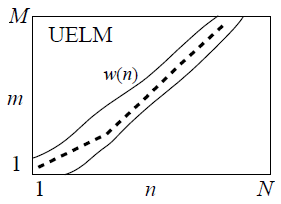
\includegraphics[width=0.3\textwidth]{Imagenes/Cap2/image052}
\end{center}
\begin{center}
\vskip -0.5cm
\caption{\small{Técnica de alineación dinámica en el tiempo UELM.}}
\label{fig:figura2.51}
{\small{Fuente: \cite{rabiner}}}
\end{center}
\end{figure}
\newpage
En \cite{rabiner2} se muestran comparaciones de estas tres variantes aplicadas en el reconocimiento de palabras aisladas y se concluye que:
\begin{enumerate}
\item[-]La variante CE2-1 genera distancias totales más grandes que la variante UE2-1.
\item[-]El algoritmo UE2-1 sirve para reducir la distancia total y para mejorar el desempeño del método.
\item[-]El algoritmo UELM se usa para aplicaciones en las cuales solamente se conoce el inicio de la palabra, por ejemplo, reconocimiento utilizando palabras concatenadas.
\end{enumerate}

Según \cite{rabiner3} se generan pequeñas pero consistentes mejoras en la exactitud de reconocimiento cuando el patrón de prueba está sobre la abscisa.

\vskip 0.5cm
En \citep{furui} se muestra que se produce menor tasa de error en la verificación de locutor cuando la palabra de menor duración se utiliza sobre la abscisa, independientemente que esta sea una palabra de prueba o de referencia.

\vskip 0.5cm
A partir de estos antecedentes, se ha optado para este trabajo de tesis el estudio de UE2-1 y UELM, a continuación explicaremos a detalle el algoritmo DTW.

\begin{enumerate}
\item[•]Restricciones de la función warping
\par
Tal como vimos anteriormente, la función warping, es una medida de la fluctuación en el eje del tiempo de los patrones del habla, la función $F = c(1), c(2),..., c(K)$, puede ser vista como una función de mapeo del patrón $A$ en el patrón $B$, quien debería conservar las estructuras lingüísticas esenciales en el patrón $A$ y viceversa, ver la Figura \ref{fig:figura2.52}.
\begin{figure}[H]
\begin{center}
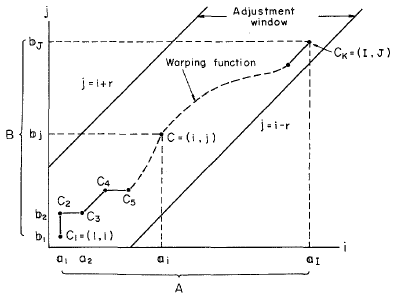
\includegraphics[width=0.45\textwidth]{Imagenes/Cap2/image053}
\end{center}
\begin{center}
\vskip -0.5cm
\caption{\small{Función warping y ventana de ajuste.}}
\label{fig:figura2.52}
{\small{Fuente: \cite{sakoe}}}
\end{center}
\end{figure}

Las restricciones de la función warping \textit{F}, son las siguientes:
\begin{enumerate}
\item[-]Condición de monoticidad:
\begin{equation}
\label{eq:ecuacion80}
i(k - 1) \leq i(k)
\text{\quad y \quad}
j(k - 1) \leq j(k)
\end{equation}

\item[-]Condición de continuidad:
\begin{equation}
\label{eq:ecuacion81}
i(k) - i(k - 1) \leq 1
\text{\quad y \quad}
j(k) - j(k - 1) \leq 1
\end{equation}
como resultado de estas restricciones, la relación entre dos puntos consecutivos está dada:
\begin{equation}
\label{eq:ecuacion82}
c(k - 1) = \left\{ \begin{array}{lcl}
(i(k),j(k - 1)) \\
\\
(i(k - 1),j(k - 1)) \\
\\
(i(k - 1), j(k)) \\
\end{array}
\right.
\end{equation}

\item[-]Condición de frontera:
\begin{equation}
\label{eq:ecuacion83}
i(1) = 1, j(1) = 1
\text{\quad y \quad}
i(K) = I, j(K) = J
\end{equation}

\item[-]Condición de ventana de ajuste:
\begin{equation}
\label{eq:ecuacion84}
\left | i(k) - j(k)) \right | \leq  r
\end{equation}
Donde $r$ es un apropiado valor entero no negativo que indica el tamaño de la ventana de ajuste, esto se debe al hecho en que las fluctuaciones en el eje del tiempo, en algunos casos nunca causan excesiva diferencia.

\item[-]Condición de slope constraint:
\par
No se deben permitir gradientes ni muy pronunciadas, ni muy suaves para la función $F$, pues puede causar desviaciones no deseables en el eje del tiempo, para gradientes pronunciadas puede causar una correspondencia no real entre un patrón muy corto y otro muy largo.
\vskip 0.5cm
La condición de slope constraint es establecida como la primera derivada de la función warping en su forma discreta, así se obliga que los valores $c(k)$ se muevan en dirección hacia adelante en el eje $i$ o en el eje $j$, consecutivamente $m$ veces, entonces no se debe permitir que $c(k)$ vaya en la misma dirección a menos que haya pasado $n$ veces por la diagonal, la intensidad efectiva del slope constraint puede ser evaluada por la siguiente medida:
\begin{equation}
\label{eq:ecuacion85}
p = \frac{n}{m}
\end{equation}

\begin{figure}[H]
\begin{center}
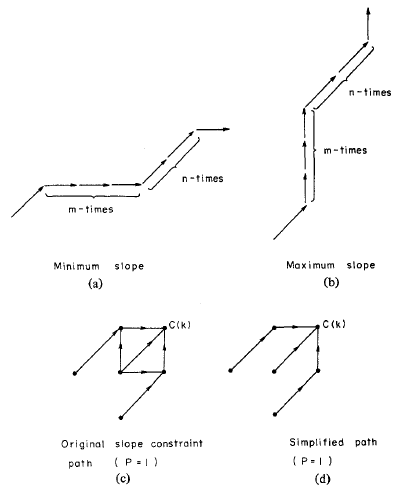
\includegraphics[width=0.55\textwidth]{Imagenes/Cap2/image054}
\end{center}
\begin{center}
\vskip -0.5cm
\caption{\small{Slope constraint en función warping.}}
\label{fig:figura2.53}
{\small{Fuente: \cite{sakoe}}}
\end{center}
\end{figure}

Cuando $P = 0$, no existen restricciones en la función warping, cuando $P = \infty$ que significa $m = 0$ la función warping está restringida a la diagonal $i = j$, si el slope constraint es muy severo, entonces la normalización en el tiempo no podrá trabajar adecuadamente y si el slope constraint es muy relajado, entonces la discriminación entre patrones de diversas categorías es degradada, por ello es deseable un valor ni muy pequeño, ni muy grande de $p$.
\end{enumerate}

\item[•]Coeficientes de peso
\par
La expresión:
\begin{equation}
\label{eq:ecuacion86}
N = \sum_{k=1}^{K}w(k)
\end{equation}
que actúa como denominador del cálculo de la distancia normalizada:
\begin{equation}
\label{eq:ecuacion87}
D(A,B) = min\left [ \frac{\sum_{k=1}^{K}d(c(k))\cdot w(k)}{\sum_{k=1}^{K}w(k)} \right ]
\end{equation}
es independiente de la función warping $F$, luego la distancia normalizada se puede escribir como:
\begin{equation}
\label{eq:ecuacion88}
D(A,B) = \frac{1}{N} min\left [ \sum_{k=1}^{K}d(c(k))\cdot w(k) \right ]
\end{equation}
y puede ser efectivamente resuelto por la técnica de programación dinámica. Existen dos definiciones de coeficientes de pesos:

\begin{enumerate}
\item[-]Forma simétrica:
\begin{equation}
\label{eq:ecuacion89}
w(k) = (i(k) - i(k - 1)) + (j(k) - j(k - 1))
\end{equation}
entonces $N = I + J$, donde $I$ y $J$ son las longitudes de los parámetros de habla $A$ y $B$ respectivamente.
\item[-]Forma asimétrica:
\begin{equation}
\label{eq:ecuacion90}
w(k) = (i(k) - i(k-1))
\end{equation}
entonces $N = I$, o equivalentemente:
\begin{equation}
\label{eq:ecuacion91}
w(k) = j(k) - j(k - 1)
\end{equation}
\vskip -0.2cm
entonces $N = J$.
\end{enumerate}

La forma simétrica significa que, si los ejes del tiempo $i$ y $j$ son continuos, entonces existirá un eje temporal: $l = i + j$ ; en la forma asimétrica se refiere a la integración a través del eje $i$ o $j$ según sea el caso. Según \citep{sakoe}, se espera que trabaje mejor la forma simétrica que la asimétrica, pues trata las partes del vector de características de igual manera, y la forma asimétrica hace alguna exclusión cuando la función warping está en dirección del eje $i$ o $j$ según sea el caso, pues $w(k)$ se reduce a cero: $c(k) = c(k-1)+(0,1)$, esto significa que algunos vectores pueden ser excluidos del análisis, pero por suerte la condición de slope constraint reduce esta situación, la diferencia de desempeño entre la forma simétrica y asimétrica puede ser gradualmente atenuada, del mismo modo que la condición de slope constraint es intensificada.

\begin{figure}[H]
\begin{center}
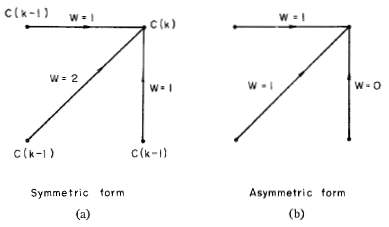
\includegraphics[width=0.5\textwidth]{Imagenes/Cap2/image055}
\end{center}
\begin{center}
\vskip -0.5cm
\caption{\small{Coeficientes de pesos para la forma simétrica y la forma asimétrica.}}
\label{fig:figura2.54}
{\small{Fuente: \cite{sakoe}}}
\end{center}
\end{figure}

\item[•]Algoritmo PD-Matching
\par
El principio de PD (Programación Dinámica) puede ser aplicado a la definición de distancia normalizada en el tiempo, el algoritmo básico es descrito como sigue:
\vskip 0.5cm
Condición inicial:
\begin{equation}
\label{eq:ecuacion92}
g_{1}(c(1)) = d(c(1))w(1)
\end{equation}
Ecuaciones PD:
\begin{equation}
\label{eq:ecuacion93}
g_{k}(c(k)) = \underset{c(k-1)}{min}[g_{k-1}(c(k - 1)) + d(c(k)w(k))]
\end{equation}
Distancia normalizada en el tiempo:
\begin{equation}
\label{eq:ecuacion94}
D(A,B) = \frac{1}{N}g_{k}(c(k))
\end{equation}
Se asume que $c(0) = (0,0)$ y $w(1) = 2$ para la forma simétrica y $w(1) = 1$ para la forma asimétrica.
\vskip 0.5cm
Pueden derivarse varios algoritmos prácticos al aplicar la forma simétrica y la forma asimétrica según la condición de slope constraint que utilicen, algunos de ellos se detallan a continuación:
\vskip 0.5cm
Para el algoritmo de la forma simétrica la condición inicial de la Ecuación \eqref{eq:ecuacion92} quedaría así:
\begin{equation}
\label{eq:ecuacion95}
g(1,1) = 2d(1,1)
\end{equation}
Ecuación PD: para $p = 0$ en su forma simétrica
\begin{equation}
\label{eq:ecuacion96}
g(i,j) = min \left\{ \begin{array}{lcl}
g(i,j - 1) + d(i,j) \\
\\
g(i - 1 , j - 1) + 2d(i,j) \\
\\
g(i - 1,j) + d(i,j) \\
\end{array}
\right.
\end{equation}
Condición de restricción (ventana de ajuste):
\begin{equation}
\label{eq:ecuacion97}
j - r \leq i \leq j + r
\end{equation}
Distancia normalizada en el tiempo:
\begin{equation}
\label{eq:ecuacion98}
D(A,B) = \frac{1}{N}g(I,J)
\end{equation}
Las ecuaciones de PD $(g(i, j))$ se calculan en orden ascendente con respecto a las coordenadas $i$ y $j$, es decir empiezan de $(i, j)$ hasta $(I, J)$.

\begin{figure}[H]
\begin{center}
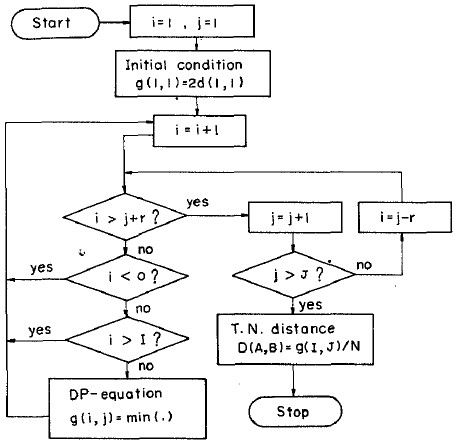
\includegraphics[width=0.5\textwidth]{Imagenes/Cap2/image056}
\end{center}
\begin{center}
\vskip -0.5cm
\caption{\small{Diagrama de flujo del algoritmo PD-Matching.}}
\label{fig:figura2.55}
{\small{Fuente: \cite{sakoe}}}
\end{center}
\end{figure}

Experimentos realizados en \citep{sakoe} muestran que el desempeño de la forma simétrica es superior al de la forma asimétrica, pero esta diferencia disminuye a medida que la condición de slope constraint es intensificada, se puede notar también que el desempeño de la forma simétrica no es afectado por un slope constraint superior a $P = 1$, por otro lado, la forma asimétrica es visiblemente mejorada por la condición de slope constraint. 
\vskip 0.5cm
Otro experimento hecho también en \citep{sakoe} evalúa el efecto de la condición de slope constraint en la forma simétrica del algoritmo PD-matching, y llega al resultado de que cuando $P = 1$ se obtiene el mejor desempeño, y en otro experimento evalúa este algoritmo con otros varios algoritmos PD propuestos por otros autores, y muestra la superioridad del algoritmo PD-matching con slope constraint $P = 1$. 
\vskip 0.5cm
En conclusión, se tiene que los mejores resultados se obtienen con la forma simétrica del algoritmo PD-matching y con una condición de slope constraint $P = 1$.

\begin{center}
\begin{table}[h!]
\centering
\vskip -0.2cm
\caption{\small{Algoritmos simétricos y asimétricos con condición de Slope Constraint P = 0, 1/2, 1, 2.}}
\label{table:tabla2}
\begin{tabular}{c}
\begin{minipage}{.9\textwidth}
\begin{center}
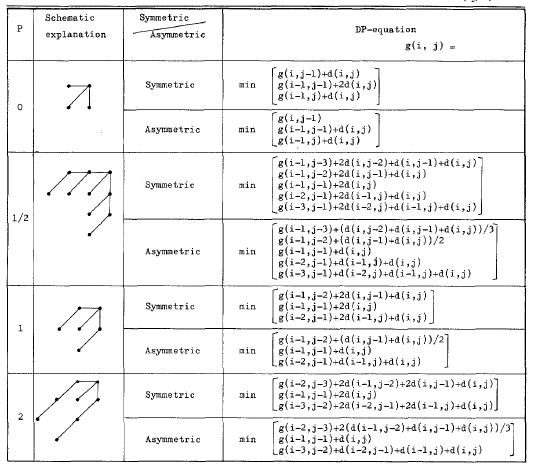
\includegraphics[width=0.85\textwidth]{Imagenes/Cap2/image057}
\end{center}
\end{minipage}
\end{tabular}
\begin{center}
\vskip 0.2cm
{\small{Fuente: \cite{sakoe}}}
\end{center}
\end{table}
\end{center}

\end{enumerate}

\item[b)]Distancias o medidas de distorsión
\par
Se hablará de \textit{medidas de distorsión} en vez de \textit{métricas} o \textit{distancias} debido a que se relajan las condiciones de simetría y desigualdad de una función de distancia con rigor matemático. Por lo tanto, no se debe utilizar el término distancia en sentido estricto, acorde a la definición expuesta; sin embargo, en la costumbre de la literatura de voz el término distancia es análogo a las medidas de distorsión.
\vskip 0.5cm
Existen varios tipos de medidas de distorsión, cada una con sus características especiales, entre ellas tenemos: \textit{Distancia Euclidiana Cuadrática, Distorsión del Error Cuadrático Medio, Distorsión del Error Cuadrático Ponderado, Distancia de Itakura, Distancia de Mahalanosis}, etc., ver en \citep{navarrete}.
\vskip 0.5cm
Para este trabajo de tesis veremos solo la Distancia Euclidiana Cuadrática y la Distancia del Error Cuadrático Medio, debido a su sencillez y poca complejidad, además de complementarse muy bien con el algoritmo DTW.

\begin{enumerate}
\item[-]Distancia Euclidiana Cuadrática
\par
La medida más conveniente y ampliamente usada para calcular distancias, es el \textit{Error Cuadrático} o \textit{Distancia Euclidiana Cuadrática}, entre dos vectores, definida como:
\begin{equation}
\label{eq:ecuacion99}
d(X_{1},X_{2}) = \left \| X_{1} - X_{2} \right \|^{2} = \sum_{j=1}^{N}(X_{1j} - X_{2j})^2
\end{equation}

\item[-]Distorsión del Error Cuadrático Medio
\par
La distorsión del \textit{Error Cuadrático Medio} (MSE) es otra de las medidas más utilizadas, en la cual la distorsión está definida por cada dimensión y se define como:
\begin{equation}
\label{eq:ecuacion100}
d(X_{1},X_{2}) = \frac{1}{N}(X_{1} - X_{2})^{T}(X_{1} - X_{2}) = \frac{1}{N}\sum_{j=1}^{N}(X_{1j} - X_{2j})^2
\end{equation}
\end{enumerate}

\vskip 0.5cm
\item[c)]Construcción del patrón de referencia
\par
El sistema de identificación de locutor se divide en dos etapas, etapa de prueba y etapa de entrenamiento. En la etapa de prueba, basta con obtener la distancia total $D_{T}$ entre los patrones de voz. Con esta distancia total y una lógica de decisión se lleva a cabo la tarea de identificar a un locutor, esta lógica de decisión se verá más adelante. Sin embargo, para construir un patrón de referencia confiable para un locutor, en la etapa de entrenamiento, es necesario conocer la función de alineamiento, $w(n)$. Como se observa en la Figura \ref{fig:figura2.52}, la función de alineamiento provee una correspondencia entre los índices de los patrones de voz. Utilizando esta correspondencia entre los patrones de voz, se puede crear un patrón de referencia $z$, simplemente promediando los vectores de los patrones de voz siguiendo la función de alineamiento, es decir:
\begin{equation}
\label{eq:ecuacion101}
z_{n} = \frac{X_{n} + Y_{w(n)}}{2}
\qquad
n=1,2,...,N
\end{equation}
En \citep{furui}, el entrenamiento se hace de la siguiente manera: Primeramente, se tienen los patrones de voz para una palabra clave, pronunciada dos veces por el locutor. Se aplica la técnica de alineación dinámica en el tiempo y se obtiene la función de alineamiento para los dos patrones de voz.
\vskip 0.5cm
Se utiliza la Ecuación \eqref{eq:ecuacion101}, para crear el primer patrón de entrenamiento. Se repite este procedimiento para la misma palabra pronunciada por tercera ocasión, pero ahora comparada contra el primer patrón de entrenamiento. Se obtiene la función de alineamiento y utilizando de nuevo la Ecuación \eqref{eq:ecuacion101}, se genera el segundo patrón de entrenamiento. Este procedimiento se sigue hasta que se ha generado el quinto patrón de entrenamiento, el cual ya se considera como un patrón de referencia. Para obtener un patrón de referencia más confiable, se utiliza un mayor número de repeticiones de la palabra clave.

\item[d)]Toma de Decisión
\par
Después de realizar la comparación de patrones es necesario tener una lógica de decisión para identificar al locutor. Este es el último paso dentro de los sistemas de reconocimiento de locutor y consiste en escoger cuál patrón de referencia (locutores conocidos) mejor corresponde con el patrón de prueba (locutor desconocido). 
\vskip 0.5cm
La forma más simple de implementar lo anterior consiste en utilizar la regla del vecino más cercano, la cual opera de la siguiente manera: se tienen $V$ patrones de referencia, $R^{i}$, $i = 1,2,...,V$, donde cada patrón de referencia representa la identidad de un locutor, y para cada patrón de referencia se obtiene la distancia total $D^{i}_{T}$, $i = 1,2,...,V$, respecto al patrón de prueba utilizando el algoritmo DTW. El patrón de referencia con la distancia mínima respecto al patrón de prueba corresponderá a la identidad del locutor.
\vskip 0.5cm
Bueno, hasta aquí se ha considerado que el sistema es de conjunto cerrado, es decir, se tienen $N$ usuarios y $N$ decisiones del sistema. Sin embargo, esto da lugar a tres respuestas del sistema: que el sistema identifique a un usuario válido, que se equivoque en identificar a un usuario y que acepte a un intruso. Dado que se requiere que el sistema no acepte intrusos, se incluyen umbrales en el sistema con el fin de aumentar la seguridad del mismo. Con estos umbrales se pretende tener un sistema de $N$ usuarios y $N+1$ decisiones.
\vskip 0.5cm
Es por ello que se utilizaran umbrales individuales para poder incluir en el sistema de identificación de locutor la respuesta \textit{no identificado}. A cada locutor o patrón de referencia le corresponde un umbral. El cálculo de los umbrales se hace mediante un método explicado en \citep{varela}, donde se define una distancia \textit{intralocutor} y una distancia \textit{interlocutor}, el primero se obtiene al comparar mediante el algoritmo DTW el patrón de referencia de un locutor contra las palabras habladas por el mismo, y el segundo se obtiene al comparar el patrón de referencia de un locutor contra las palabras habladas por la base de datos de locutores sin incluir las palabras que pertenecen al locutor del cual se usa el patrón de referencia. 
\vskip 0.5cm
Se supone que tanto el conjunto de distancias intralocutor, como el de distancias interlocutor pueden ser aproximados por distribuciones de probabilidad normal como se muestra en la Figura \ref{fig:figura2.57}.

\begin{figure}[H]
\begin{center}
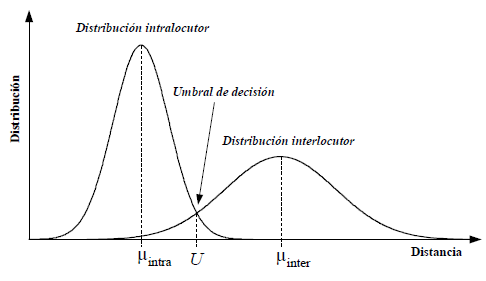
\includegraphics[width=0.5\textwidth]{Imagenes/Cap2/image058}
\end{center}
\begin{center}
\vskip -0.5cm
\caption{\small{Distribuciones de probabilidad de las distancias intralocutor e interlocutor.}}
\label{fig:figura2.57}
{\small{Fuente: \cite{varela}}}
\end{center}
\end{figure}
\vskip -0.5cm
El umbral $U$ es el punto en donde el área bajo la curva de la distribución intralocutor desde $U$ a más infinito es igual al área bajo la curva de la distribución interlocutor desde menos infinito a $U$, es decir, el punto donde la probabilidad de que el sistema responda \textit{no identificado} es igual a la probabilidad de que exista una \textit{falsa identificación}. Las distribuciones de probabilidad normal de la Figura \ref{fig:figura2.57}. están dadas por la siguiente ecuación:
\begin{equation}
\label{eq:ecuacion102}
P(D) = \frac{1}{\sqrt{2 \pi \sigma }}e^{\frac{(D - \mu)^{2}}{2 \sigma^{2}}}
\end{equation}
Donde $\mu$ es la media y $\sigma$ es la desviación estándar. El umbral $U$ se calcula a partir de las siguientes ecuaciones:
\begin{equation}
\label{eq:ecuacion103}
U - \mu_{int ra} = n \sigma_{int ra}
\end{equation}
\begin{equation}
\label{eq:ecuacion104}
\mu_{int er} - U = n \sigma_{int er}
\end{equation}
despejando $n$ de las Ecuaciones \eqref{eq:ecuacion103} y \eqref{eq:ecuacion104} e igualando se obtiene el umbral $U$ de la siguiente forma:
\begin{equation}
\label{eq:ecuacion105}
U = \frac{\sigma_{int ra}\mu_{int er} + \sigma_{int er}\mu_{int ra}}{\sigma_{int ra} + \sigma_{int er}}
\end{equation}
Si es que se tienen 10 patrones de referencia (10 usuarios del sistema), es necesario calcular un umbral por cada patrón de referencia, es decir:
\begin{equation}
\label{eq:ecuacion106}
U_{i} = \frac{\sigma^{int ra}_{i} \mu^{int er}_{i} + \sigma^{int er}_{i} \mu^{int ra}_{i}}{\sigma^{int ra}_{i} + \sigma^{int er}_{i}}
\qquad
i = 1,2,...,9
\end{equation}
\end{enumerate}
\vskip 0.5cm
\section{Método de la investigación}
\subsection{Diseño de la investigación}
De acuerdo al fin que persigue, el presente trabajo es una investigación aplicada. Por otro lado, de acuerdo al diseño de contrastación de la hipótesis es una investigación experimental.

\subsection{Variables de estudio}
\begin{enumerate}
\item[•]\textbf{Variable dependiente:} Control de acceso a una vivienda.
\item[•]\textbf{Variable independiente:} Sistema de seguridad por reconocimiento de voz.
\end{enumerate}

El factor de medida para el control de acceso a una vivienda mediante el reconocimiento de voz consiste en el tiempo de respuesta y la tasa de precisión en el reconocimiento que se obtengan de los resultados experimentales.

\subsection{Métodos y procedimientos para la recolección de datos}
Para recolectar los datos se harán grabaciones a 10 personas escogidas aleatoriamente, para esto se contará con el micrófono del dispositivo móvil y el del computador. El procedimiento a emplear será darle a cada persona una lista de dos comandos de voz (\textit{Abrir} y su \textit{Nombre}), las cuales, al ser leídas, serán grabadas. El nivel de ruido de la grabación deberá ser moderado.

\subsection{Población y muestra}
Siendo una investigación experimental, la determinación de la muestra se basa en los antecedentes \cite{eyra} y \cite{varela} debido a que estás investigaciones son de caso similar y en la experiencia del autor.
\subsubsection{Población}
\begin{enumerate}
\item[•]\textbf{Área:} Audios de señales de voz.
\item[•]\textbf{Categoría:} Palabras de idioma español.
\item[•]\textbf{Subcategoría:} Hombres con edad promedio de 23 años.
\end{enumerate}
La población es infinita para esta investigación, debido al número infinito de formas distintas en que una señal de voz puede ser capturada. Se tomarán en cuenta audios donde se muestren señales de voz de palabras en español habladas por hombres con edad promedio de 23 años.

\subsubsection{Muestra}
La muestra estará conformada por un conjunto de 800 audios dividido entre los comandos de voz \textit{Abrir} y los \textit{Nombres de los Usuarios} (Edwin, Carlos, Josué, Édison, Gerson, Nizama, Anthony, Jhordan, Renzo y Franchesco), los cuales serán las palabras claves de acceso para 10 miembros de la vivienda, por lo que estará agrupada por el conjunto de estos 11 comandos de voz.
\vskip 0.5cm
Dado que la población de señales de voz es infinita, se optó por usar un muestreo aletorio simple para poblaciones desconocidas con un nivel de confianza del 95\% y un error de muestreo del 3.5\%.

\begin{equation}
\label{eq:ecuacion}
n = \frac{z^{2}pq}{e^2}
\end{equation}

En el que:
\begin{enumerate}
\item[•]$n$ = Tamaño de muestra.
\item[•]$z$ = Coeficiente de confiabilidad 95\% al que corresponde (1.96).
\item[•]$pq$ = Varianza de la población, ponemos la varianza mayor posible porque a mayor varianza hará falta una muestra mayor (0.25).
\item[•]$e$ = Error muestral 3.5\% (0.035).
\end{enumerate}

\subsection{Método de estudio}
Para llegar a los objetivos propuestos, el desarrollo de la investigación comprendió las siguientes etapas:
\begin{enumerate}
\item[a)]Análisis del problema de los sistemas de control de acceso en la ciudad de Trujillo, en el Perú y el mundo, comprendiendo la situación actual y el levantamiento de los principales casos de éxito.
\item[b)]Formulación del problema principal de la investigación y justificación de la importancia de su solución.
\item[c)]Recopilación de herramientas, técnicas y métodos acústicos matemáticos y físicos de la voz para identificar y autenticar a los dueños de la vivienda.
\item[d)]Levantamiento de los diferentes temas necesarios para la elaboración de la investigación.
\item[e)]Diseño e implementación del software de reconocimiento de voz.
\item[f)]Diseño y construcción del hardware capaz de ser controlado a través del protocolo de red inalámbrica 802.11g.
\item[g)]Integración de las dos partes mencionadas anteriormente, así como la ejecución de pruebas para su correcto funcionamiento.
\item[h)]La implementación de todo el sistema en un ambiente real.
\item[i)]Realización del reporte de incidencias ocurridas mientras estaba en uso el sistema.
\item[i)]Para el análisis de resultados, se pretende usar la técnica de Chi-Cuadrado de Pearson para dos variables nominales, a través de esta técnica se puede conocer la relación de dependencia de nuestras variables con Identificación Correcta, Falsa Identificación y No Identificación métricas usadas conmumente para evaluar la calidad de nuestro sistema de reconocimiento de voz.
\end{enumerate}

\subsection{Análisis estadístico de los datos}
Para efectuar el análisis estadístico de los datos se hará la prueba de independencia Chi- Cuadrado de Pearson para dos variables nominales.
\vskip 0.5cm
El uso de esta prueba es que permite contrastar los resultados de una prueba o método propuesto, determinando si dos cualidades o variables referidas a individuos de una población están relacionadas. 

\subsection{Esquema general del proyecto}
En la Figura \ref{fig:figura2.58} se muestra el diagrama de bloques para el esquema general de este proyecto, primero la señal voz es capturada por el micrófono del dispositivo móvil, en el caso de que se habilite la opción de filtrado de ruido en el sistema, el micrófono del computador capturara la señal de ruido, luego el sistema se encargará de procesar y analizar la señal de voz (con la señal de ruido, si es que la hubiera) y dependiendo de la respuesta del reconocimiento de dicha señal este le enviará o no una señal al microcontrolador que controla el acceso, activando o no la cerradura eléctrica.
\vskip 0.5cm
\begin{figure}[H]
\begin{center}
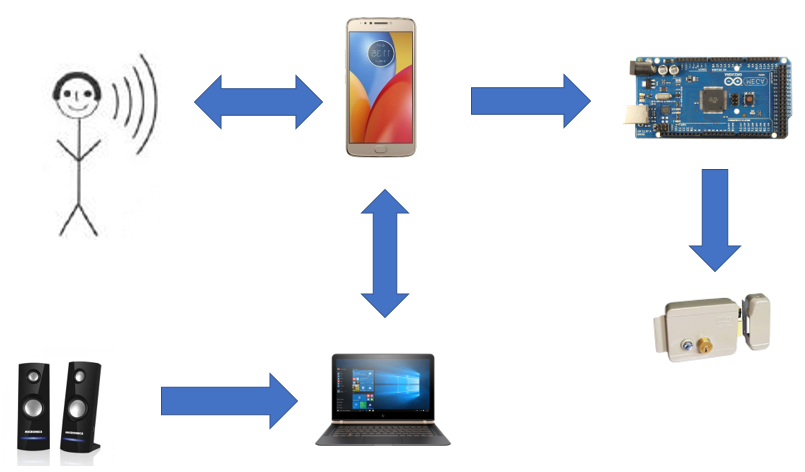
\includegraphics[width=0.8\textwidth]{Imagenes/Cap2/image059}
\end{center}
\begin{center}
\vskip -0.5cm
\caption{\small{Diagrama de bloques general del proyecto.}}
\label{fig:figura2.58}
{\small{Fuente: Elaboración propia}}
\end{center}
\end{figure}